\chapter{Aspects of quarkonium physics}
\label{chap:pquarkonia}

\minitoc

\myepigraph{At least we can all agree on one thing: The people who see
  the dress as white are utterly, completely wrong.}{Adam Rogers, in \textit{The Science of Why No One Agrees on the Color of This Dress},
  www.wired.com}


\section{Quarkonium production in vacuum}
\label{sec:production}
% Because of several factors, the quarkonium production is a
% long-standing riddle.
Quarkonia were first studied extensively at
$e^{+}e^{-}$ colliders. For example, the BABAR detector at Stanford (USA)
and BELLE at Tsukuba (Japan) have analysed hundreds of inverse
femtobarns of $e^{+}e^{-}$ events at the centre-of-mass energy of
a $\Upsilon(4S)$ at rest (and above), to study $B$ meson production and other
heavy flavour related processes. Among these, the spectroscopy of
heavy flavour and quarkonia has been studied with great
precision~\cite{nora}.
%  In this Section, I will
% prevent myself from saying that no-one is able to understand
% quarkonium production (there \textit{is} hope).
The quarkonium production mechanisms are however, still debated.
 I will start with a
discussion of the allowed decay processes for quarkonia, by virtue of
the Okubo-Zweig-Iizuka (OZI) rule~\cite{Okubo:1963fa,Iizuka:1966fk,Zweig:570209}; this will
help me to give a naive view of the possible production modes, by
simply turning around the decay process. Then, I will discuss what
the binding of two quarks means in terms of
spectroscopy and decay, before moving to an experimental review of
some interesting results, and finish with an increase in temperature to
see to what risks a quarkonium exposes itself when wandering in nuclear
matter. Beginning with an experimental review, I will make a detour in
charmonium physics, before moving to a discussion of available results in
the bottomonium sector.


\subsection{Introductory remarks: the OZI rule}
\label{sec:OZI}
In Chapter~\ref{chap:pqcd}, I have mentioned the existence of new
resonances in the 1970's dilepton spectrum of $e^{+}e^{-}$
colliders. One of the particularities of these new \Jpsi and $\Upsilon$ peaks
is their very narrow signal shape, compared to what was usually known in the
lower part of the mass spectrum (except for the $\phi$ meson, which is
$s\bar{s}$). 
\\
This is a consequence of the OZI
rule. For heavy quark-antiquark states $\psi$ of the same flavour $s\bar{s},\,
c\bar{c},\, b\bar{b}$, the possible decay processes are: electromagnetic
annihilation or hadronic decays. The rate of the electromagnetic
annihilation quarkonium is of a typical order
$\alpha_{QED}^{2}$~\cite{gatto}. On the other hand, the hadronic 
decay is mediated by the strong interaction. So at first, one can say
that quarkonia will either decay strongly via the hadronic channel, or
via QED-mediated processes, seemingly with a smaller rate (as
$\alpha_{QED} < \alpha_{S}$). For a chosen $\psi$ state having
spin 1, and odd parity, and the hadrons being colour singlets, there
are several constraints to the QCD mediated decay:
\begin{itemize}
\item[-] the final state being composed of colour singlets
  (e.g. pions), the decay cannot be mediated by one gluon (which is a
  colour octet\footnote{I did not mention it when discussing group
    theory, but the existence of a ninth, colour-singlet gluon would
    make QCD = U(3), and the interaction length would be infinite: no confinement.});
\item[-] the two-gluon decay is also prohibited, since a vector
  meson can not decay into two massless vector gluons, by virtue of
  the charge conjugation ($C$) quantum number conservation;
\item[-] but, the decay to three gluons would be allowed, as well as
  decays into more gluons.
\end{itemize}



With these considerations, the quarkonium hadronic decay is driven by
$\alpha_{S}^{3}$ and higher orders. For the $\phi$ meson, the decay into two kaons is
favoured by the conservation of the strangeness content. The OZI rule
then states that decays where quark lines do not connect the initial
and the final state are suppressed. One such example of OZI-suppressed
diagrams is presented in Figure~\ref{fig:OZI}.
\\
\begin{figure}[h]
\begin{center}
  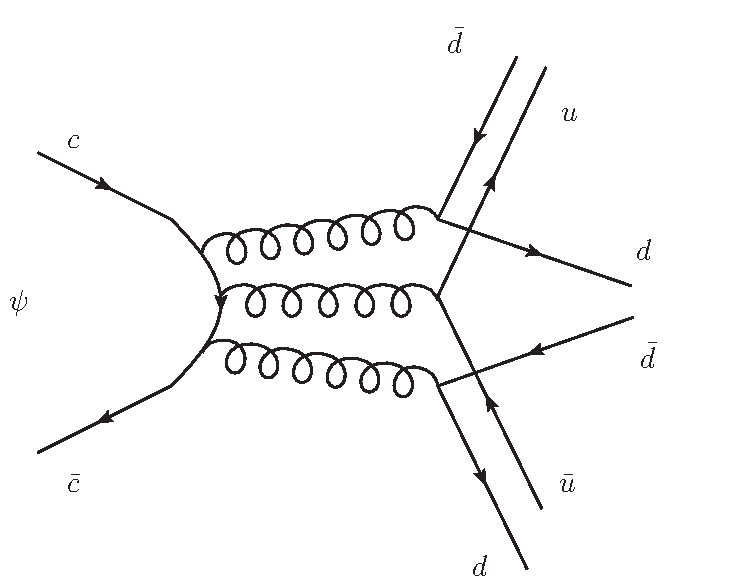
\includegraphics[width=0.6\textwidth]{Chapters/pQuarkonia/OZI.pdf}
 \caption{A \Jpsi decay to three gluons, suppressed by the OZI rule.}
 \label{fig:OZI}
\end{center}
\end{figure}
\\
What we have seen applies to $\phi$ mesons, as well as to % be leaving the $\phi$ on the side for now, and on
heavy quarkonium states, our main interest. The \Jpsi for instance, has a mass of $m_{\Jpsi} = 3.096~
\GeV/c^{2}$, which is smaller than the twice the $D^{0}$ mass. This
means that decays of the kind $\Jpsi \to D^{0}\bar{D}^{0}$ are
kinematically ruled out, leaving only QED annihilation and
OZI-forbidden hadronic decays. This results in an experimental width
of the order of 10 \keV, which was smaller than the experimental
resolution at that time! It is the combination of the $D$ meson observation above the
\Jpsi mass and the narrow width of $\psi$ states which definitely
identified the new resonances and hadrons as from a new quark flavour.
\\
\subsection{Production mechanisms: the hard part}
\label{sec:models}
One of the important questions of this Chapter (the question is likely to remain
unanswered), is whether we know what is (are) the production
mechanism(s) of quarkonia. 
I will restrict myself to the case of hadron-hadron collisions, but
there is also quarkonium production in electron-positron annihilation,
photoproduction, DIS. These channels have been very fertile and would require a whole separate
review, which I will not engage in.
\\
The hadron-hadron interaction can produce at tree level in QCD a pair of quark and
antiquark:
\begin{itemize}
% \item[-] a QED-mediated process, $q\bar{q} \to
% \gamma^{\star}/Z \to Q\bar{Q}$, which is usually called Drell-Yan,
\item[-] via QCD-annihilation $q\bar{q} \to Q\bar{Q}$,
\item[-] via gluon fusion and splitting, $gg \to Q\bar{Q}$.
\end{itemize}
 At the LHC, the large distribution of gluons inside each proton makes the gluon
 fusion the \textit{dominant} channel for large $Q^{2}$ and small-$x$ processes, which leads us to consider gluon
 fusion as the dominant initial state for quarkonium production in our
 review. Then comes the issue of the quantum
 numbers in the final state.
\\
We have J$^{PC}$ = 1$^{--}$ for \Jpsi and \PgU. From the OZI rule we
have seen that the decay of \Jpsi into one gluon is impossible
kinematically; Additionally, the two-gluon decay would
violate the charge conjugation parity, as the left part is C-odd, and
the right part is C-even.
\\
Strictly speaking, it is possible to turn the OZI rule around and
realise that the only way to produce a quarkonium with the correct
quantum numbers is by the
interaction of at least three gluons. A process with three gluons in the initial state
has a too small rate, that could not account for the measured
\Jpsi rate.

So at LHC energies, gluon fusion is dominant \textit{and} the
pre-quarkonium state formed has to emit gluons to equilibrate its
degrees of freedom of angular momentum and/or colour. This in some sense resembles
hadronisation, although we do not know what is the colour of the initial
state; Rather, nothing prevents the gluon fusion to produce a white or
a coloured $Q\bar{Q}$ pair at the partonic level a priori. It is only
afterwards when the pair hadronises that the colour is
equilibrated.


There are various ways to recover the proper quantum numbers for each
quarkonium wave function: in fact, when expanding to ever higher
orders of the perturbative $\alpha_{S}$ expansion, one finds an
infinity of terms contributing to quarkonium production. Some
models have been proposed to describe the production processes: 
\begin{itemize}
\item[-] The Colour Singlet Model (CSM)~\cite{CSM} assumes that quarkonia are directly
  produced with the `good' quantum numbers, i.e. the one they have
  when they decay: this poses strong
  constraints on either the kinematics or the total rate for producing
  a given state, as can be seen in Figure~\ref{fig:CDF_CSM};
\item[-] The Colour Octet Model (COM)~\cite{Braaten:1994vv} suggests that quarkonium production via
  a pre-resonant colour octet intermediate state would in fact matter,
  to the point where these extra terms may
  become dominant. In this point of view the CSM alone can not
  account for the spectrum of a given quarkonium and its integrated
  cross section at the same time;
\item[-] Non-Relativistic QCD (NRQCD)~\cite{nrqcd} tries to unify CSM and COM:
  Stating that a hard process can be factorised from the long distance
  hadronisation
  part, it details the amplitudes of quarkonium production as an
  expansion of terms involving a short distance (hard part) resembling
  the CSM, and a long distance matrix element (LDME) containing
  the color octet contributions. Given the fact that both quarks are heavy,
  they can be treated non-relativistically in the quarkonium rest
  frame;%, thus giving credit to the factorisation hypothesis;
\item[-] Finally, the Colour
  Evaporation Model (CEM)~\cite{Amundson:1996qr} suggests a quarkonium production following
  dynamics comparable to that of heavy flavour hadron pairs
  ($D\bar{D}$ in the case of charmonium, \textit{etc.}). % The model has
  % been given fame in the days of Tevatron and HERA days, when CSM was
  % strongly failing.
  In this case, the colour equilibration is treated
  as a nonperturbative process, related to the hadronisation phase.
\end{itemize}



% Before going into the details of each model, I would like to point out
% some group-theoretical aspect which helped in my personal
% understanding of the 'divide' between CSM and COM advocates.

% Making use of the fact that quarks form a triplet in the fundamental
% representation of QCD, one could construct the following equation:
% \begin{equation}
% \mathbf{3\times\bar{3} = 1 \oplus 8}
% \end{equation}
% Adding the quark degrees of freedom together to make a
% $Q\bar{Q}$ wavefunction, one can construct either a colour singlet or
% octet. All final state objects observed are colour singlets of course,
% so the existence of colour octet states or terms has to be temporary:
% the question whether this is a long scale or short scale process is
% relevant in this discussion, and that's where (I believe) the 'divide'
% stands between CSM and COM lies. That would seem trivial to
% experimentalists, but when making a detailed QCD calculation of the
% $Q\bar{Q}$ amplitude including leading and next-to-leading order terms
% for example, one may ask himself whether the colour octets can live
% outside the tree-level, parton world, or not.
% \\
% Authors Baier and Ruckl have argued in the past~\cite{CSM} that the quarkonium
% object could be produced dominantly as a colour singlet, the octet
% terms being suppressed with higher powers of $\alpha_{S}$. This led to what
% is known nowadays as the colour singlet model. In this framework, the $Q\bar{Q}$
% pair is produced in the correct quantum numbers at the partonic tree
% level, so a very small number of diagrams are needed to compute the
% amplitude. Only the binding between quarks remains non-perturbative. Unfortunately, the
% colour singlet model (CSM) has issues, some of which I want to detail here.
% \\
The \pt(\Jpsi) spectrum measured at CDF in $p\bar{p}$
collisions does not match the colour singlet (LO), neither
qualitatively nor quantitatively~\cite{CDFpsi}. At tree level (LO), the expected
\pt-spectrum behaves according to the CSM as $\pt^{-8}$, which disagrees strongly
with the experimental measurement of CDF, as one can see on both
panels of Figure~\ref{fig:CDF_CSM}.

\begin{figure}
\begin{center}
  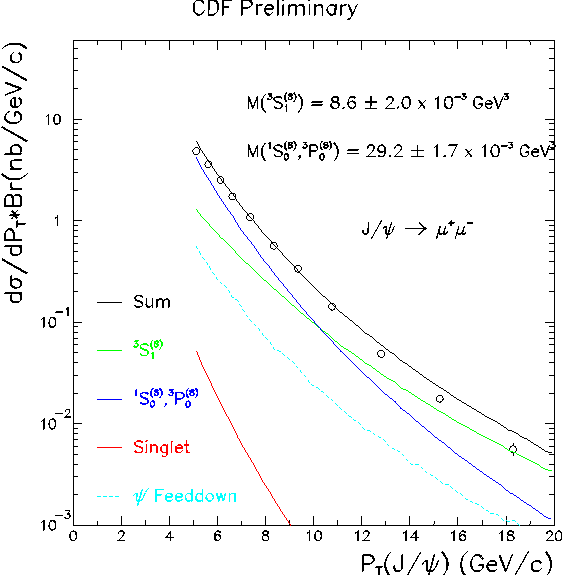
\includegraphics[width=0.45\textwidth]{Chapters/pQuarkonia/CDFpsi1S.pdf}
  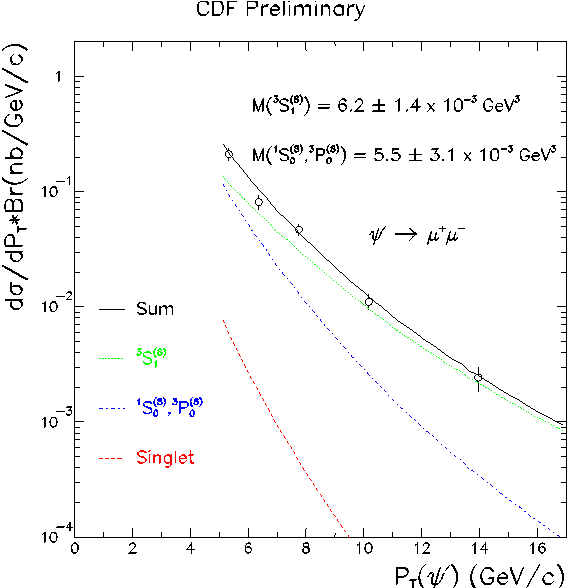
\includegraphics[width=0.45\textwidth]{Chapters/pQuarkonia/CDFpsi2S.pdf}
  \caption{Charmonium momentum distributions from
    CDF~\cite{CDFpsi}. Left, the \Jpsi spectrum compared to LO CSM and
    additional colour octet terms. Right: same computation for
    $\psi(2S)$.}
  \label{fig:CDF_CSM}
\end{center}
\end{figure}

 The left hand side specifically treats the
case of \Jpsi, and the $\psi(2S)$ case is presented on the right hand
side of
Figure~\ref{fig:CDF_CSM}. In the colour singlet hypothesis,
% poses strong constraints on the branching fractions from higher states
% (further referred to as feed-down fractions). Indeed, since
the quarkonium $\psi$ is produced from a gluon fusion process $gg \to ? \to \psi +
X$ with a colour singlet  wavefunction $\psi$ and its
allowed quantum numbers are that of $\eta$ ($^{1}S_{0}$) or
$chi_{0,2}$ ($^{3}P_{0,2}$). This would mean that all \Jpsi\ come from
radiative decays $\chi_{c} \to \Jpsi\gamma$, and all $\psi(2S)$ come
from $b$ decays. A measurement of the prompt $\psi(2S)$ rate compared
to the non-prompt $b \to \psi(2S)$ rate, by the CDF collaboration in 1994, has shown
that the theoretical prediciton were in an order of magnitude of
disagreement with the experimental data~\cite{CDF:1994aa}.

% This did not 'kill' the CSM
% instantly, as one starts to imagine that refined NLO QCD corrections come into
% play. We shall see that CSM predictions to higher orders are still
% used today by experiments to compare with their quarkonium
% data. Still, one can argue that a higher order term can only be
% smaller than the previous order, otherwise the perturbative limit is
% not satisfied and the whole expansion is meaningless. However, the
% criticism arguing whether the CSM really has a sound theoretical basis
% is out of the scope of this here discussion.







\subsection{Quarkonium spectroscopy}
\label{sec:spectro}
Associating a quark and an antiquark of the same flavour (often called
hidden heavy flavour) in a bound state will
result in a constrained spectroscopy. One can find common examples of
simple semi-classical systems (treated quantum mechanically, but where
the dynamics are non-relativistic) such as the positronium system or
the hydrogen atom, or the H$_{2}$ molecule, that would produce
comparable classifications of energy levels. Of course the quantum formalism
would be that of QED, and since we are interested in QCD in this case, the analogy
has some limitations. Nonetheless, one can model an effective
quarkonium potential of the form that was used in
Equation~\ref{eq:potential} and solve the Schrödinger equation, to
extract a spectroscopy, i.e. energy levels that can be compared to
experimental data by simply measuring the mass of each resonance
discovered. 
\\
\begin{figure}
\begin{center}
  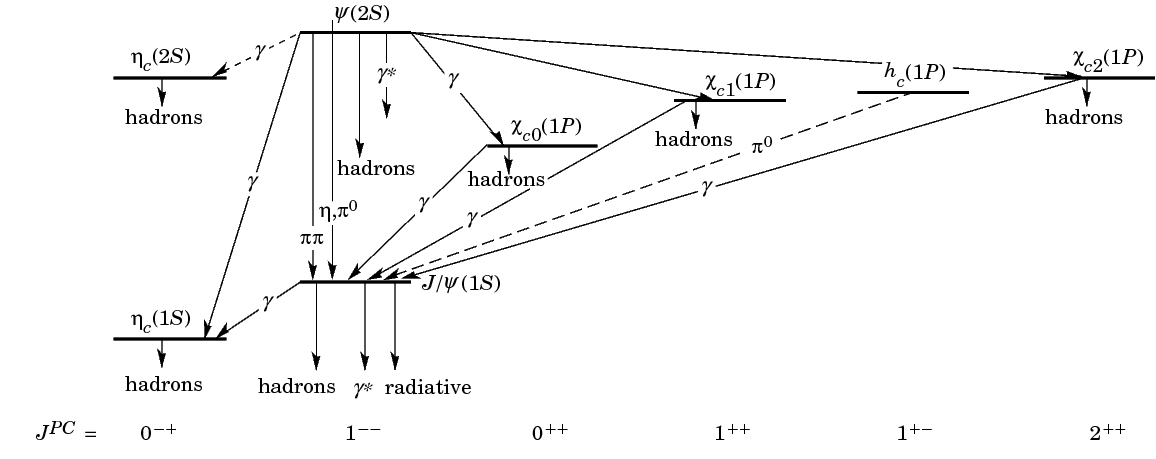
\includegraphics[width=0.9\textwidth]{Chapters/pQuarkonia/charmonia.png}
  \caption{Charmonium spectroscopy. The abscissae are J$^{PC}$ indices
  (spin, parity, charge conjugation). From~\cite{spectro}.}
  \label{fig:charmonium}
\end{center}
\end{figure}
\\
For both charm and beauty, the spectroscopy begins with a ground state
with quantum numbers $n=0$, $L=0$, $S=0$, $J=0$, which is usually
identified as an $\eta_{c}$ or an $\eta_{b}$ meson. One finds higher energy bound states of various quantum numbers up
to the $D^{0}\bar{D}^{0}$ 
threshold or the $B^{0}\bar{B}^{0}$ threshold, for charm and beauty
respectively. Above the threshold, the inital $Q\bar{Q}$
system contains enough rest energy to decay dominantly in $D$ or
$B$ mesons. Resonances existing above this threshold are far wider, as for
example $\Upsilon(4S), \Upsilon(5S), \Upsilon(6S)$. For these, all
OZI-favored hadronic transitions are measurable, hence their very
large width (for example $\Gamma(\Upsilon(4S)) / \Gamma(\Upsilon(nS))
\approx 500$ for n < 4).

The charmonium spectroscopy is depicted in Figure~\ref{fig:charmonium}. All
states appearing are below the $D\bar{D}$ threshold. Other states have
been discovered, for which a very consequent review is done by the
Quarkonium Working Group~\cite{nora}. The simplest possible
transitions are drawn with arrows, and correspond to radiative
deexcitations (dipolar electric E1 transitions) or emission of one or
several light hadrons.


\begin{figure}[htb]
\begin{center}
  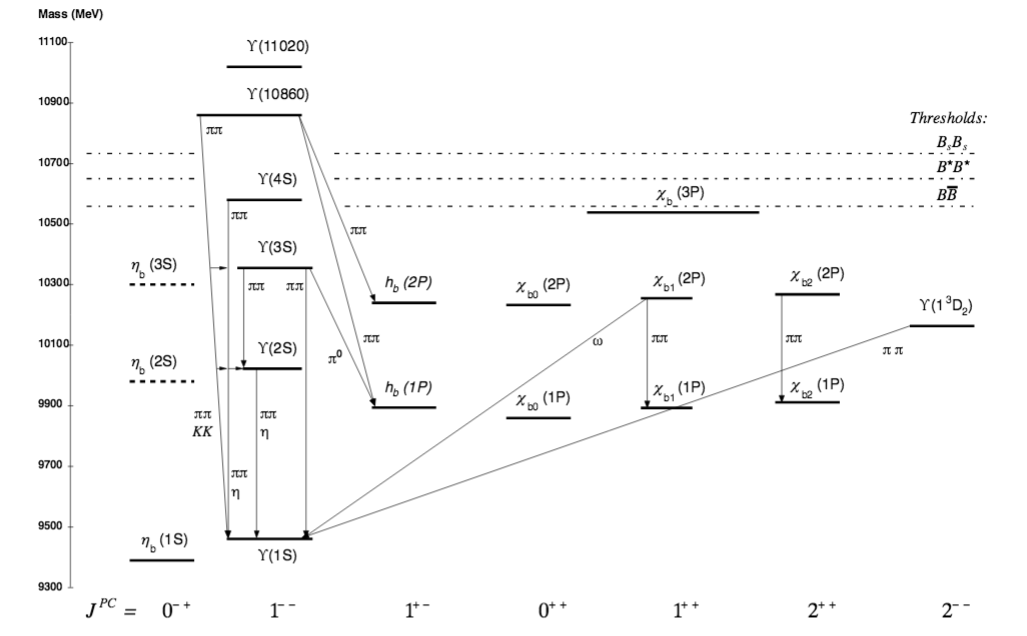
\includegraphics[width=0.7\textwidth]{Chapters/pQuarkonia/bottomonium.png}
  \caption{Bottomonium spectroscopy. The abscissae are J$^{PC}$ indices
  (spin, parity, charge conjugation). The vertical axis, not
  displayed, would represent increasing theoretical rest masses. From~\cite{spectro}.}
  \label{fig:bottomonium}
\end{center}
\end{figure}
\vspace{0.3cm}
For bottomonia, the picture is somewhat more complicated by the larger
gap between the ground state mass and the $B\bar{B}$ threshold. As one
can see on Figure~\ref{fig:bottomonium}, the spectroscopy resembles
that of charmonium, as expected. The recently discovered $\chi_b(3P)$
state~\cite{chib3p,chib3p_lhcb} does not appear in this picture and
would stand between $\chi_b(2P)$ and the $B\bar{B}$ threshold.
\\
The transitions from excited states to lower levels of the bottomonium
family, called feed-down
fractions, are summed up in Figure~\ref{fig:hermine}. These
fractions represent the ratio of cross sections for bottomonium states
decaying into another, as a function of the product \PgU~\pt. Here are of
interest the radiative E1 transitions $\chi(mP) \to \PgU(nS)$, with $n\leq
m-1$ and the hadronic transitions $\PgU(nS) \to \PgU(n'S)$, with $n'
\leq n-1$. As we can anticipate, the kinematics of the decay constrain the
total \PgU~decay
rate, and this has in the past led to misconceptions regarding
feed-down fractions of \PgUa~from higher states. These feed-down
fractions may be crucial to interpret the suppression 
pattern of quarkonium modification or suppression in heavy ion collisions.


\begin{figure}[htb]
\begin{center}
  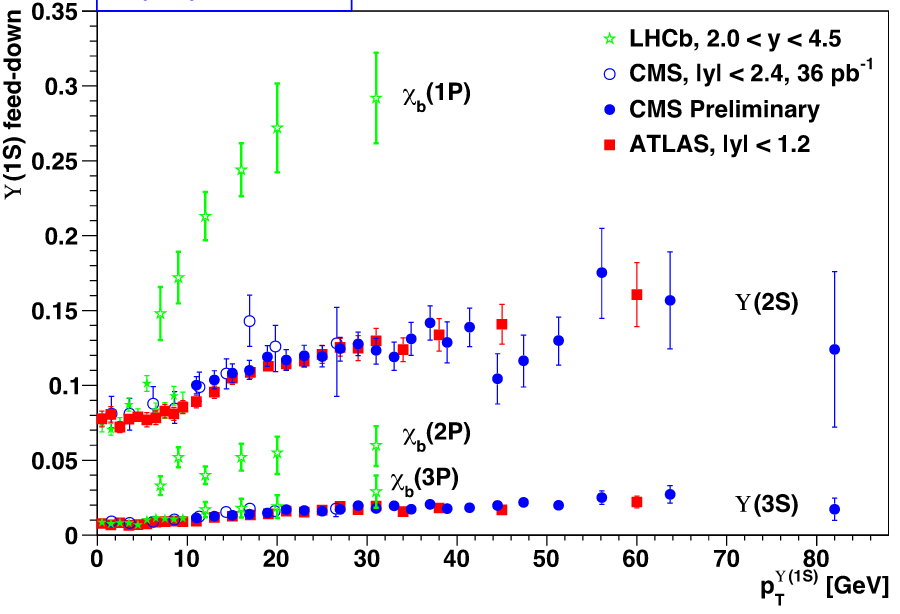
\includegraphics[width=0.8\textwidth]{Chapters/pQuarkonia/feeddown.png}
  \caption{Feed-down fractions of excited bottomonia to \PgUa, as a
    function of the transverse momentum of the \PgUa\ meson. From~\cite{hermine}}
  \label{fig:hermine}
\end{center}
\end{figure}


\vspace{0.5em}
\begin{center}
  \fbox{
    \parbox{0.9\textwidth}
    {\textsf {In this section the basis of our understanding of
        quarkonium production in vacuum was presented. The
        experimental data from Tevatron provided a long standing
        puzzle to a theoretical formulation that would reproduce the
        data. However, with newer high-luminosity experiments such as
        the LHC or future experiments, a larger understanding of
        quarkonium production in $pp$ can be possible.}}} 
\end{center}



\section{Charmonia in nuclear matter}
% In vacuum, the charmonium states are very well measured. There are
% many reviews of the charmonium physics. Experimentally, one of the
% causes of resurgence in charmonium physics was the impossibility
% to match the \Jpsi spectrum from Tevatron data to leading order (LO)
% and next-to-leading order (NLO) calculations.

% Nowadays the frameowrk of NRQCD works quite well at reproducing parts
% of the spectrum of charmonium states. The LHC has produced impressive
% results for the \pt spectrum of \Jpsi, $psi'$ and $\chi_{c}$ states,
% as well as measurements of exotic states as $X(3872)$.
\subsection{At the SPS}

% Starting with NA3 collaboration data, the $x_{F}$ dependence of \Jpsi
% production is measured with good precision. Later measurements at HERA
% in $ep$ and $eA$ collisions presented interesting constraints to the gluon PDF:
% there, quarkonium photoproduction is highly-driven by the kinematics
% of the gluon in the nucleon or the nucleus, and the comparison of both
% gives a good constraint on $xg$.

The
CERN SPS fixed target experiments NA38, NA50 and NA60 investigated the
charmonium sector in various heavy ion systems ($pp$, $p$-A, A-B, A-A,
with various ions A and B), to look for the onset of suppression~\cite{Baglin:1990iv,Abreu:1997jh,Abreu:2000xe,Abreu:2000ni,Alessandro:2004ap,jpsiNA60}. In all cases, the
experiment could use multiple targets, allowing for a precise scan of
the energy density dependence of the collision. 

Each experiment reconstructed dimuon invariant mass pairs in the
charmonium region and around, to measure the signal and background
constributions. The \Jpsi and $\psi(2S)$ cross sections were extracted
from other same-charge background dimuon sources % such as open charm, Drell-Yan and
% combinatorics from $\pi$ and $K$ decays~\cite{Alessandro:2004ap}.
In order to measure the centrality,
one could record the energy deposited in zero degree calorimeters
(ZDC) or using the multiplicity in a nearby silicon tracking device, and
later use a Glauber model calculation to extract an effective length $L$ of
nuclear material seen by the probe. The Drell-Yan cross section
$\sigma(A+B \to \mu^+\mu^-)$, measured
around the \Jpsi peak (2.9 < $m_{\mu\mu}$ < 4.5~\unitMass)~\cite{Alessandro:2004ap}, is used as a
reference in all collision setups to compare with the~\Jpsi cross
section, as is shown on Figure~\ref{fig:na60}.



\begin{figure}[htb]
\begin{center}
  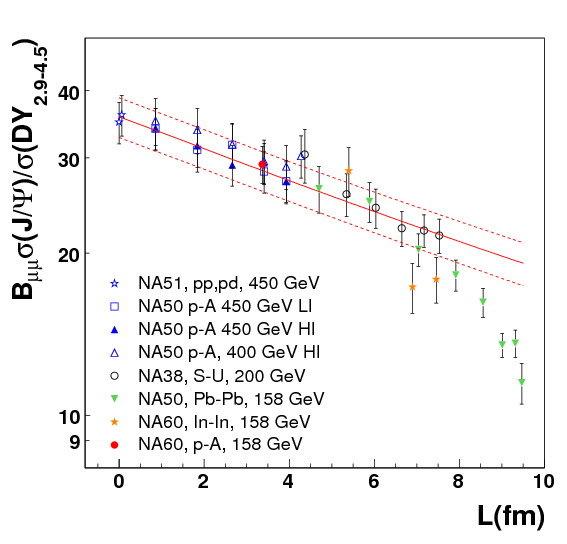
\includegraphics[width=0.6\textwidth]{Chapters/pQuarkonia/NA60.png}
  \caption{\Jpsi suppression from SPS experiments as a function of
    nuclear length $L$. From~\cite{compilSPS}.}
  \label{fig:na60}
\end{center}
\end{figure}



The green points represent what was called an 'anomalous'
suppression, in the sense that above $L = 7$ fm the observed data does not
conform to pure nuclear absorption. The  nuclear absorption is
estimated using a Woods-Saxon nuclear distribution fitted to data,
exhibiting an absorption cross section of $\sigma_{\rm {abs}}= 4.18 \pm
0.35$ mb.%  This suppression can be further investigated by separating
% charmonium states \Jpsi and $\psi(2S)$. Figure~\ref{fig:psi2SPS}




% In itself, Figure~\ref{fig:na60} is not a definite proof of melting in
% heavy ions collisions. First, the observed suppression for \Jpsi
% contains feed-down from $\psi(2S)$ and $\chi_{c}$, for which the plot
% does not tell the suppression pattern. Second, the nuclear length $L$
% compares different collision geometries in pA, AA (A = Pb, In, \textit{etc.})
% and hence might be inadequate. A further measurement of more than just
% \Jpsi, extending at higher number of participants or at higher
% energies is needed to disentangle nuclear absorption from
% QGP. 
\subsection{At RHIC}

Studies to find the effects of deconfinement progressed at Brookhaven
with the start of RHIC (Relativisitc Heavy Ion Collider) operation
in 2000.
The charmonium system was measured there in pp collisions at \s\ = 500
GeV, in deuteron-gold (dAu) and gold-gold (AuAu) collisions at \snn\ =
200 GeV.

The dependence of charmonium suppression was investigated there as a
function of transverse momentum, rapidity and centrality percentiles,
the latter instead of nuclear matter length. The centrality is again obtained via a
Glauber model calculation, which in the case of the PHENIX experiment,
is correlated to the collected charge in the Beam Beam
Counters (BBC). A complete review of centrality measurements for AuAu
and dAu collisions with the PHENIX detector from RHIC is available
in~\cite{centralityRHIC}.
\begin{figure}
\begin{center}
  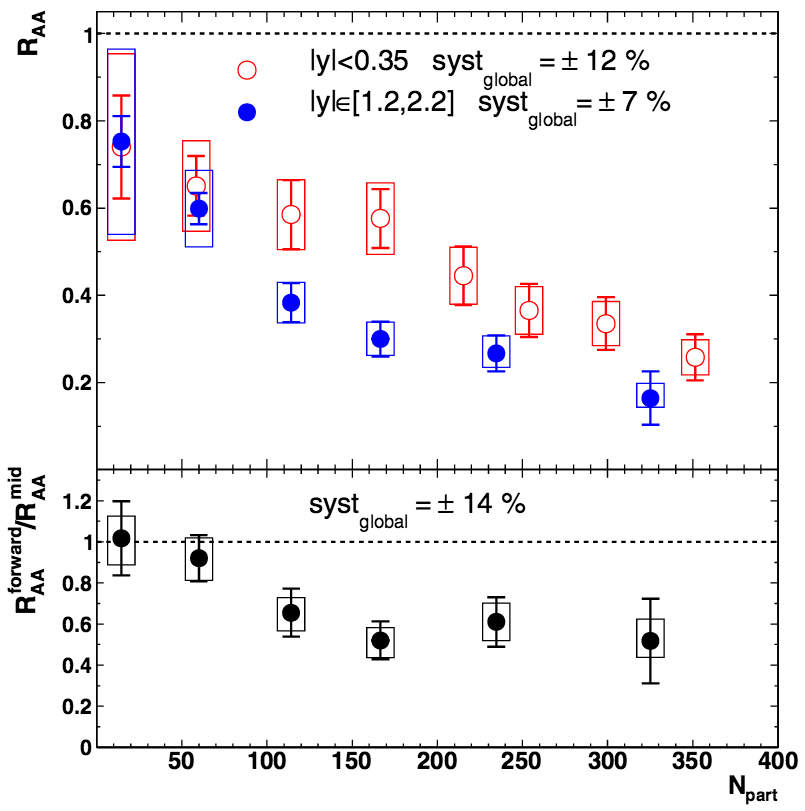
\includegraphics[width=0.5\textwidth]{Chapters/pQuarkonia/Phenix_raa_centrality.png}
  \caption{\Jpsi suppression in AuAu collisions at \snn~=~200 GeV from PHENIX at RHIC, as a function of
    centrality. Two rapidity regions are shown: central (open symbols),
    forward (closed symbols). From~\cite{jpsiphenix}.}
  \label{fig:phenixnpart}
\end{center}
\end{figure}
Figure~\ref{fig:phenixnpart} shows the centrality dependence of \Jpsi
suppression at \snn\ = 200 GeV from PHENIX. The \Jpsi yields are
measured in the central region (open symbols) and in the forward
direction (blue). This seems to show that the \Jpsi is more suppressed
at RHIC in the forward direction, which is counterintuitive: indeed
the energy density is expected to be higher in the central rapidity
region, which would lead to more suppression in the central arm.

% As to compare with the anomalous suppression of SPS, the situation now
% worsens with this new anomaly. In contrast, 
The \Jpsi suppression from fixed target experiments at SPS energies was
probing regions of the Bjorken-$x \approx 0.1$, a region where the gluon density is
relatively unmodified in nuclei, compared to the $x$ regime of PHENIX
measurements (smaller $x$ values, typically $10^{-3} < x <
10^{-2}$). In this small-$x$ region, the gluon density can suffer a depletion
(\textit{shadowing}) effect in nuclei, resulting in a \Jpsi yield
slightly affected downwards. The nuclear modification factor in dAu
from PHENIX~\cite{jpsiphenixdAu}, $R_{dAu}$ is presented in
Figure~\ref{fig:dAuphenix} (left) and
presents indeed some suppression in the p-going direction, which is in
this case positive rapidities.




\begin{figure}[th]
\begin{center}
  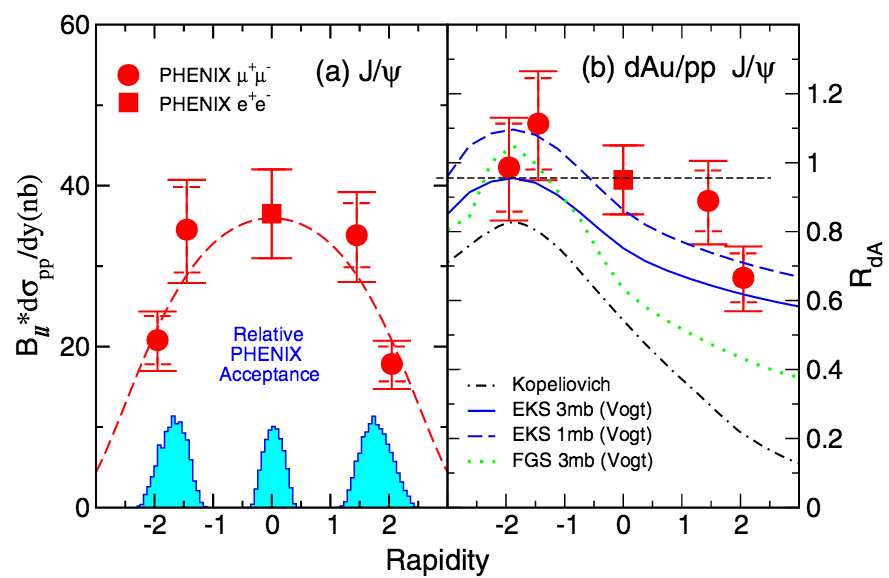
\includegraphics[width=0.5\textwidth]{Chapters/pQuarkonia/Phenix_rday.png}
  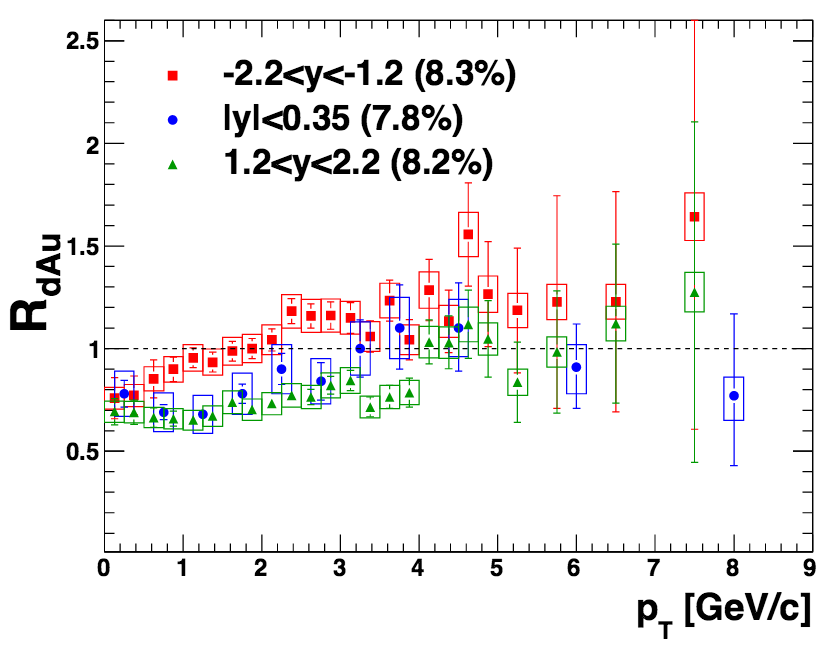
\includegraphics[width=0.42\textwidth]{Chapters/pQuarkonia/Phenix_rdapt.png}
  \caption{\Jpsi suppression in dAu collisions at \snn~=~200 GeV
    measured by the PHENIX experiment at RHIC, as a function of
    \Jpsi rapidity (left) and transverse momentum (right). From~\cite{jpsiphenixdAuy,jpsiphenixdAupt}.}
  \label{fig:dAuphenix}
\end{center}
\end{figure}



One can also notice on Figure~\ref{fig:dAuphenix} (right) the \pt
dependence of the \Jpsi dAu suppression. The \Jpsi seems to be
slightly suppressed in low transverse momenta. This \pt-dependent
measurement of the suppression in dAu need to be completed with a
measurement involving two ions, to see if any additional suppression
is thus also reflected in the AA \pt\ spectrum.


\begin{figure}[th]
\begin{center}
  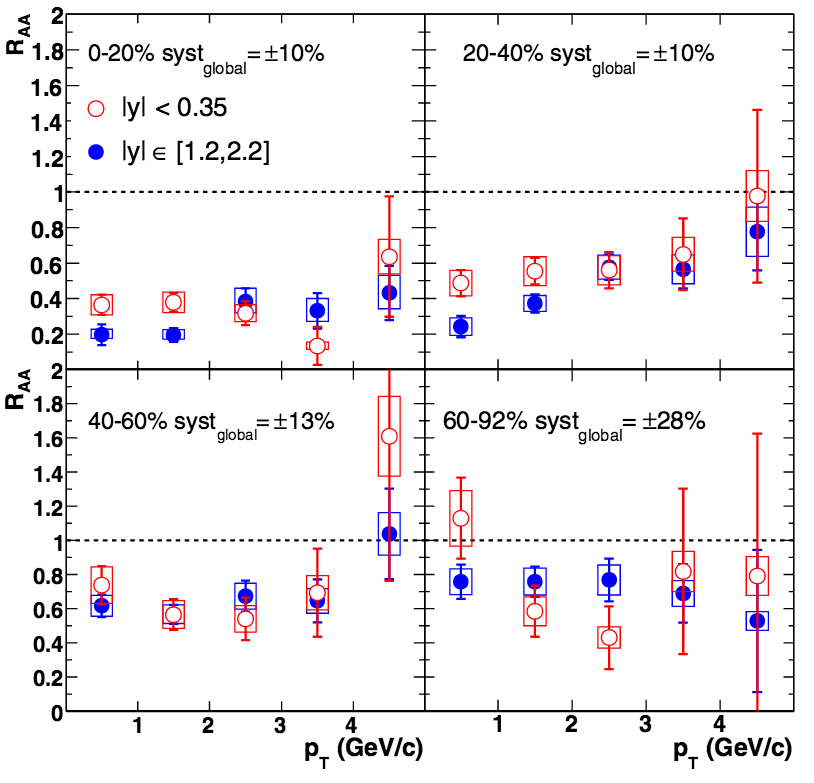
\includegraphics[width=0.8\textwidth]{Chapters/pQuarkonia/Phenix_raa_pt.png}
  \caption{\Jpsi suppression in AuAu collisions at \snn~=~200 GeV
    measured with the PHENIX experiment at RHIC, as a function of
    \Jpsi transverse momentum. The four panels from top left to bottom
    right correspond to decreasing centrality classes. Open symbols:
    central rapidity, closed symbols: forward rapidity. From~\cite{jpsiphenix}.}
  \label{fig:AuAuphenixpt}
\end{center}
\end{figure}


Thanks to RHIC data, the suppreesion of \Jpsi in AuAu and $d$Au has been
clearly measured, to finally reach a lowest suppression point of
approximately \RAA $\approx$ 0.2 in
 low-\pt central AuAu collisions. In Figure~\ref{fig:AuAuphenixpt} the
 \pt-dependence of \Jpsi in AuAu collisions is presented with various
 centrality classes. The suppression seems to be stronger in high centrality,
 low-\pt events. However, a mild difference between forward and
 central rapidities is observed, and could be explained by more
 nuclear absorption setting in at forward rapidities, or a
 possible gluon shadowing effect. 

\clearpage
\subsection{At the LHC}


At the LHC, the energy in the centre-of-mass for PbPb collisions is \snn~=
2.76 TeV for the first operation period (Run1, up to 2013). The center
of mass energy in pPb is \snn~= 5.02 TeV, while pp data was taken at
\s~= 2.76, 7, 8 TeV.
The ALICE and CMS experiments have measured \Jpsi~yields with high
precision in pp, pPb and PbPb, yielding several suprises. First of
all, the suppression measured at ALICE is much less pronounced at low
transverse momentum than in the RHIC data, as is shown on
Figure~\ref{fig:aliceJpsi} (left). This plot also has \Jpsi data from
the CMS collaboration (prompt \Jpsi, \pt > 6.5 \GeVc) in the central
rapidity region. The right hand side of Figure~\ref{fig:aliceJpsi} has the
rapidity dependence of inclusive \Jpsi suppression in PbPb, exhibiting
less suppression at midrapidity than at RHIC
(cf. Figure~\ref{fig:AuAuphenixpt}), and a stronger suppression when
going to higher rapidity ranges.

\begin{figure}[h]
\begin{center}
  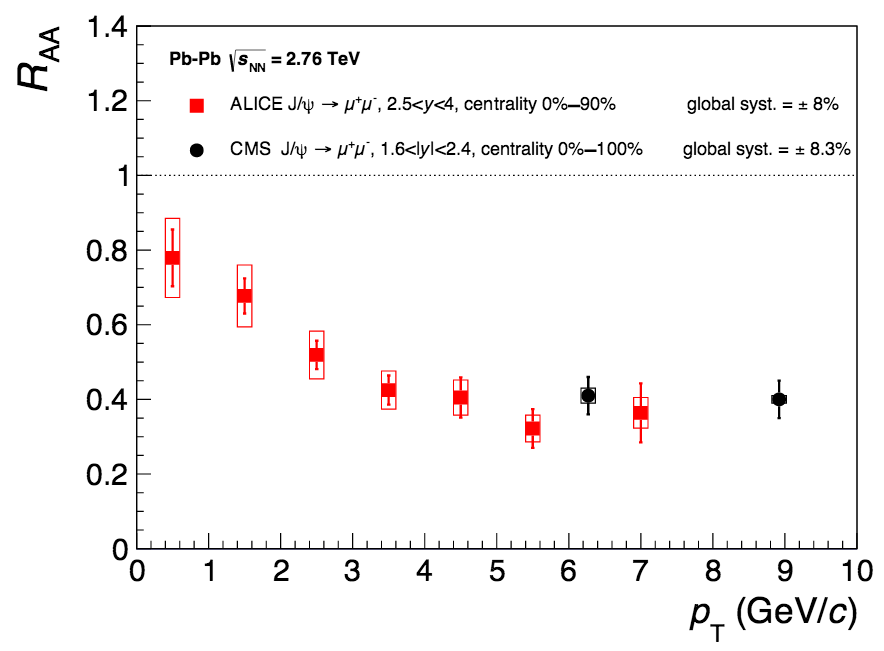
\includegraphics[width=0.48\textwidth]{Chapters/pQuarkonia/Aliceraapsipt.png}
  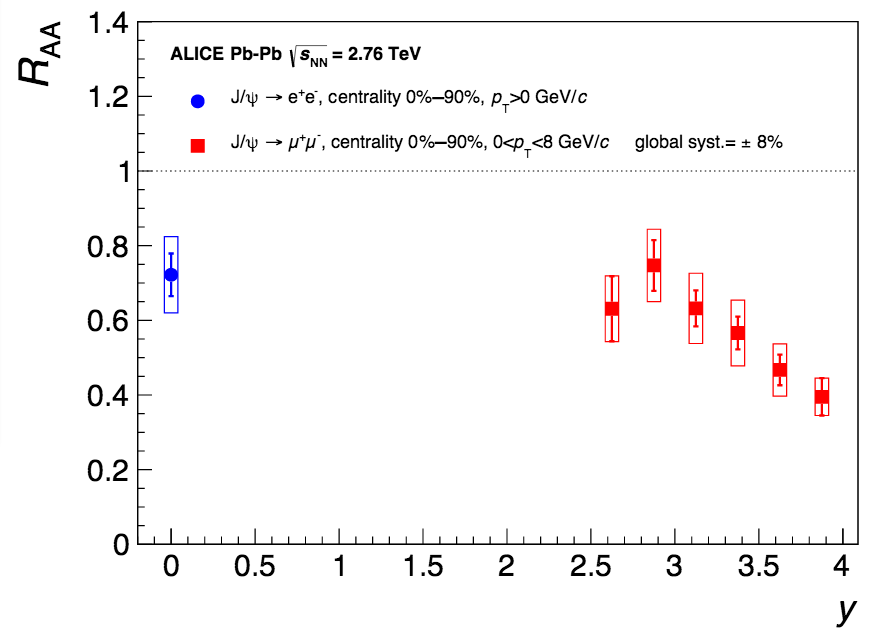
\includegraphics[width=0.48\textwidth]{Chapters/pQuarkonia/Alicepsipbpby.png}
  \caption{\Jpsi suppression in PbPb collisions at LHC energies, as a function of
    the \Jpsi \pt in ALICE forward data and CMS data (left), and as a
    function of \Jpsi rapidity with ALICE (right). Red squares:
    forward rapidity, blue circles: central rapidity. Black squares:
    CMS high \pt data. From~\cite{jpsiALICE}.}
  \label{fig:aliceJpsi}
\end{center}
\end{figure}



On Figure~\ref{fig:alicenpart}, the
centrality dependence is presented, and appears saturating at $\RAA \sim$ 0.65 from \Npart\ = 100. When comparing with RHIC results,
this looks like a strong enhancement, or a much weaker
suppression. Models accounting for statistical recombination of
decorrelated charm quarks~\cite{BraunMunzinger:2000px,Grandchamp:2002wp} into \Jpsi\ suggest that at LHC energies, the
energy density is such that about 100 $c\bar{c}$ pairs are produced in
central PbPb events, leading to a large probability for these quarks
to combine in the hadronic freeze out phase in a \Jpsi\ (or $\psi(2S)$)
state, hence populating the spectrum and reducing the observed
suppression in this phase space region.
\begin{figure}[h]
\begin{center}
  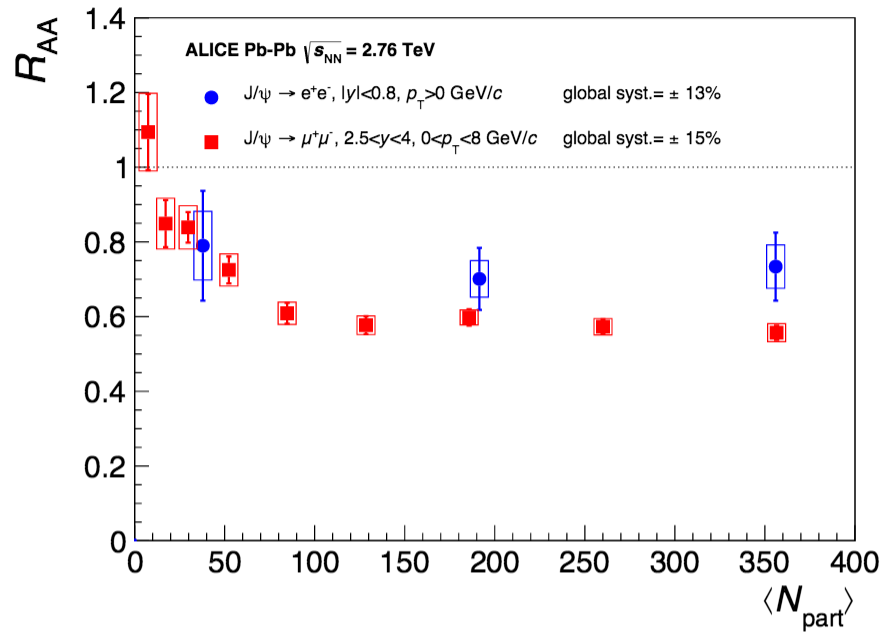
\includegraphics[width=0.65\textwidth]{Chapters/pQuarkonia/Aliceraanpartpsi.png}
  \caption{\Jpsi suppression in PbPb collisions from ALICE, as a function of
    the centrality of the collision. Red squares:
    forward rapidity, blue circles: central rapidity. From~\cite{jpsiALICE}.}
  \label{fig:alicenpart}
\end{center}
\end{figure}



The CMS collaboration has published a \pt, rapidity and centrality dependent \Jpsi
result~\cite{torsten} for high \pt \Jpsi (prompt and non-prompt,
i.e. coming from secondary displaced vertices). The \RAA was further
 recently updated with higher statistics in pp data in~\cite{12014} and is
presented in Figure~\ref{fig:CMSpsi}.
\begin{figure}[h]
\begin{center}
  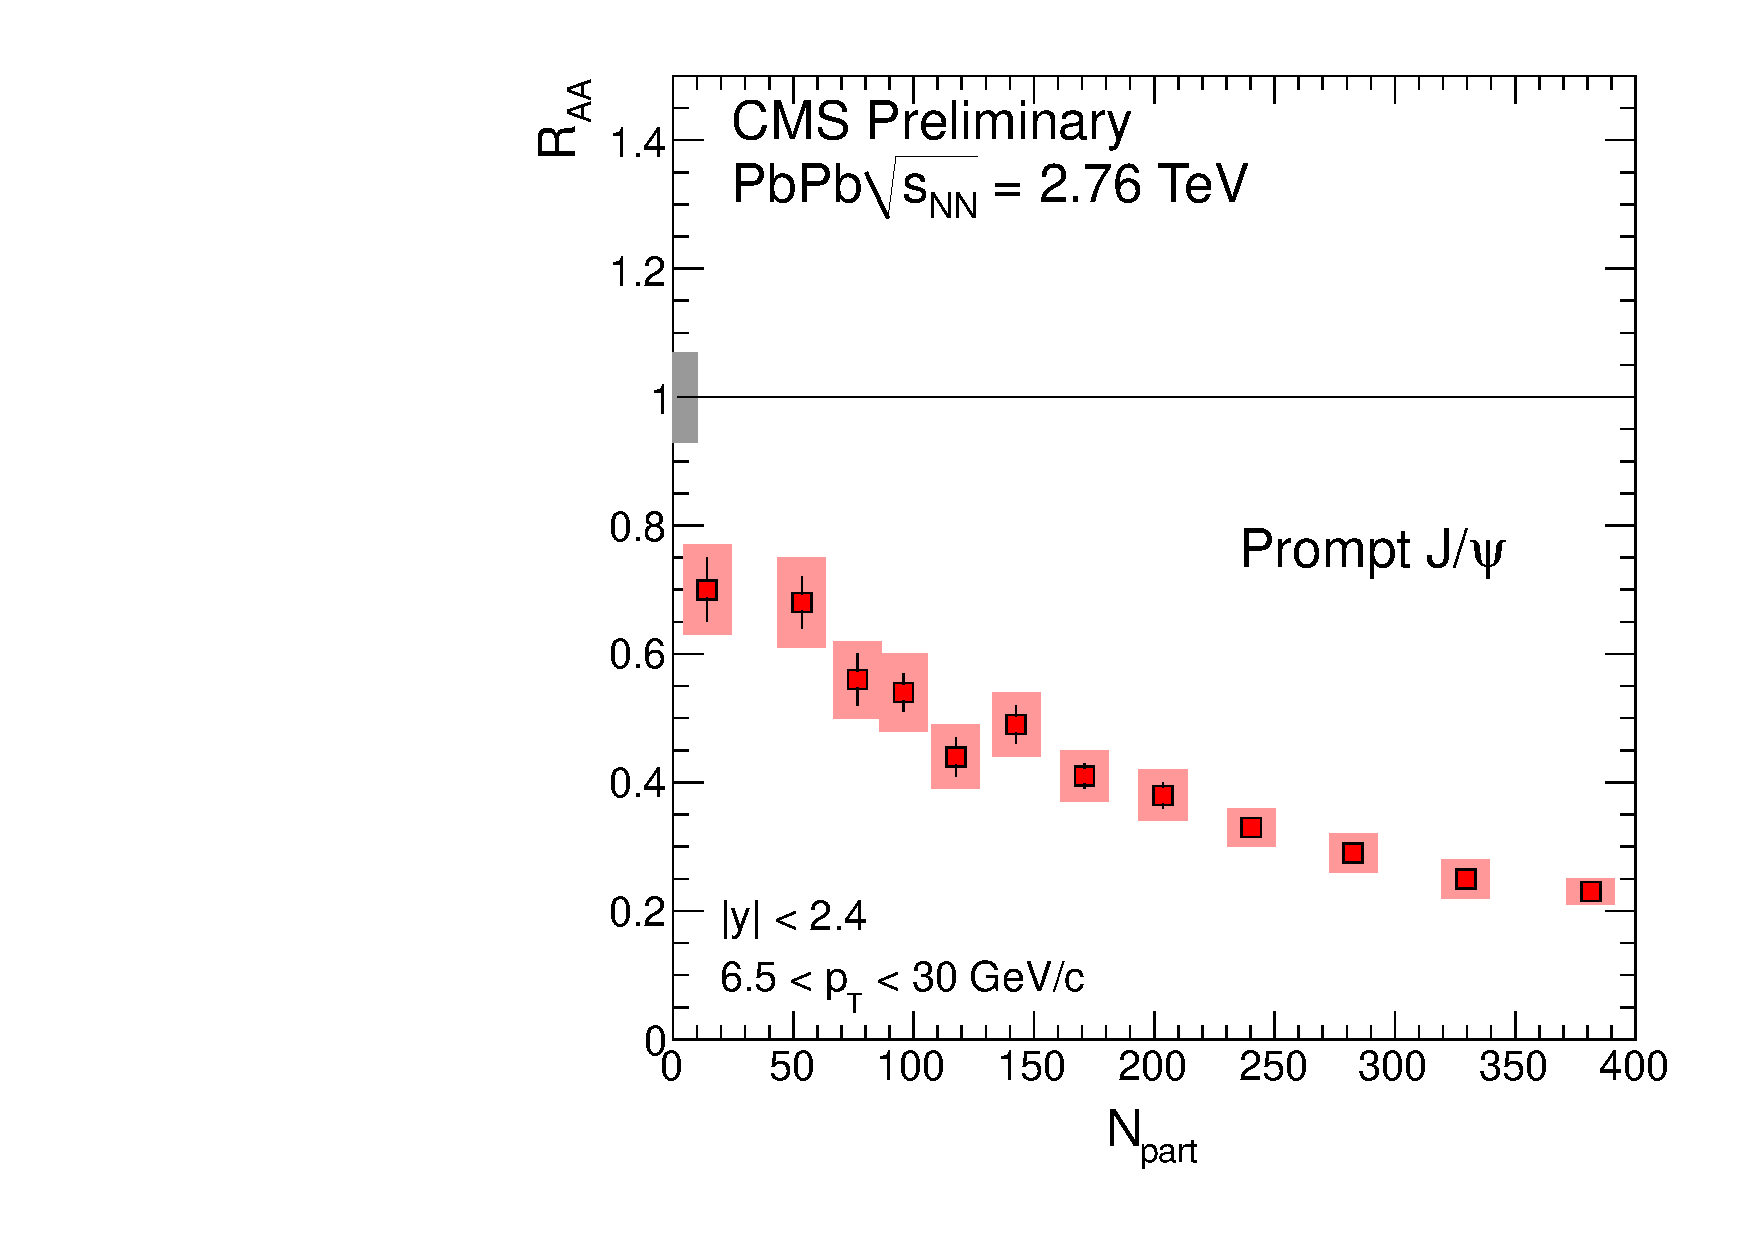
\includegraphics[width=0.7\textwidth]{Chapters/pQuarkonia/CMSPromptJpsi.pdf}
  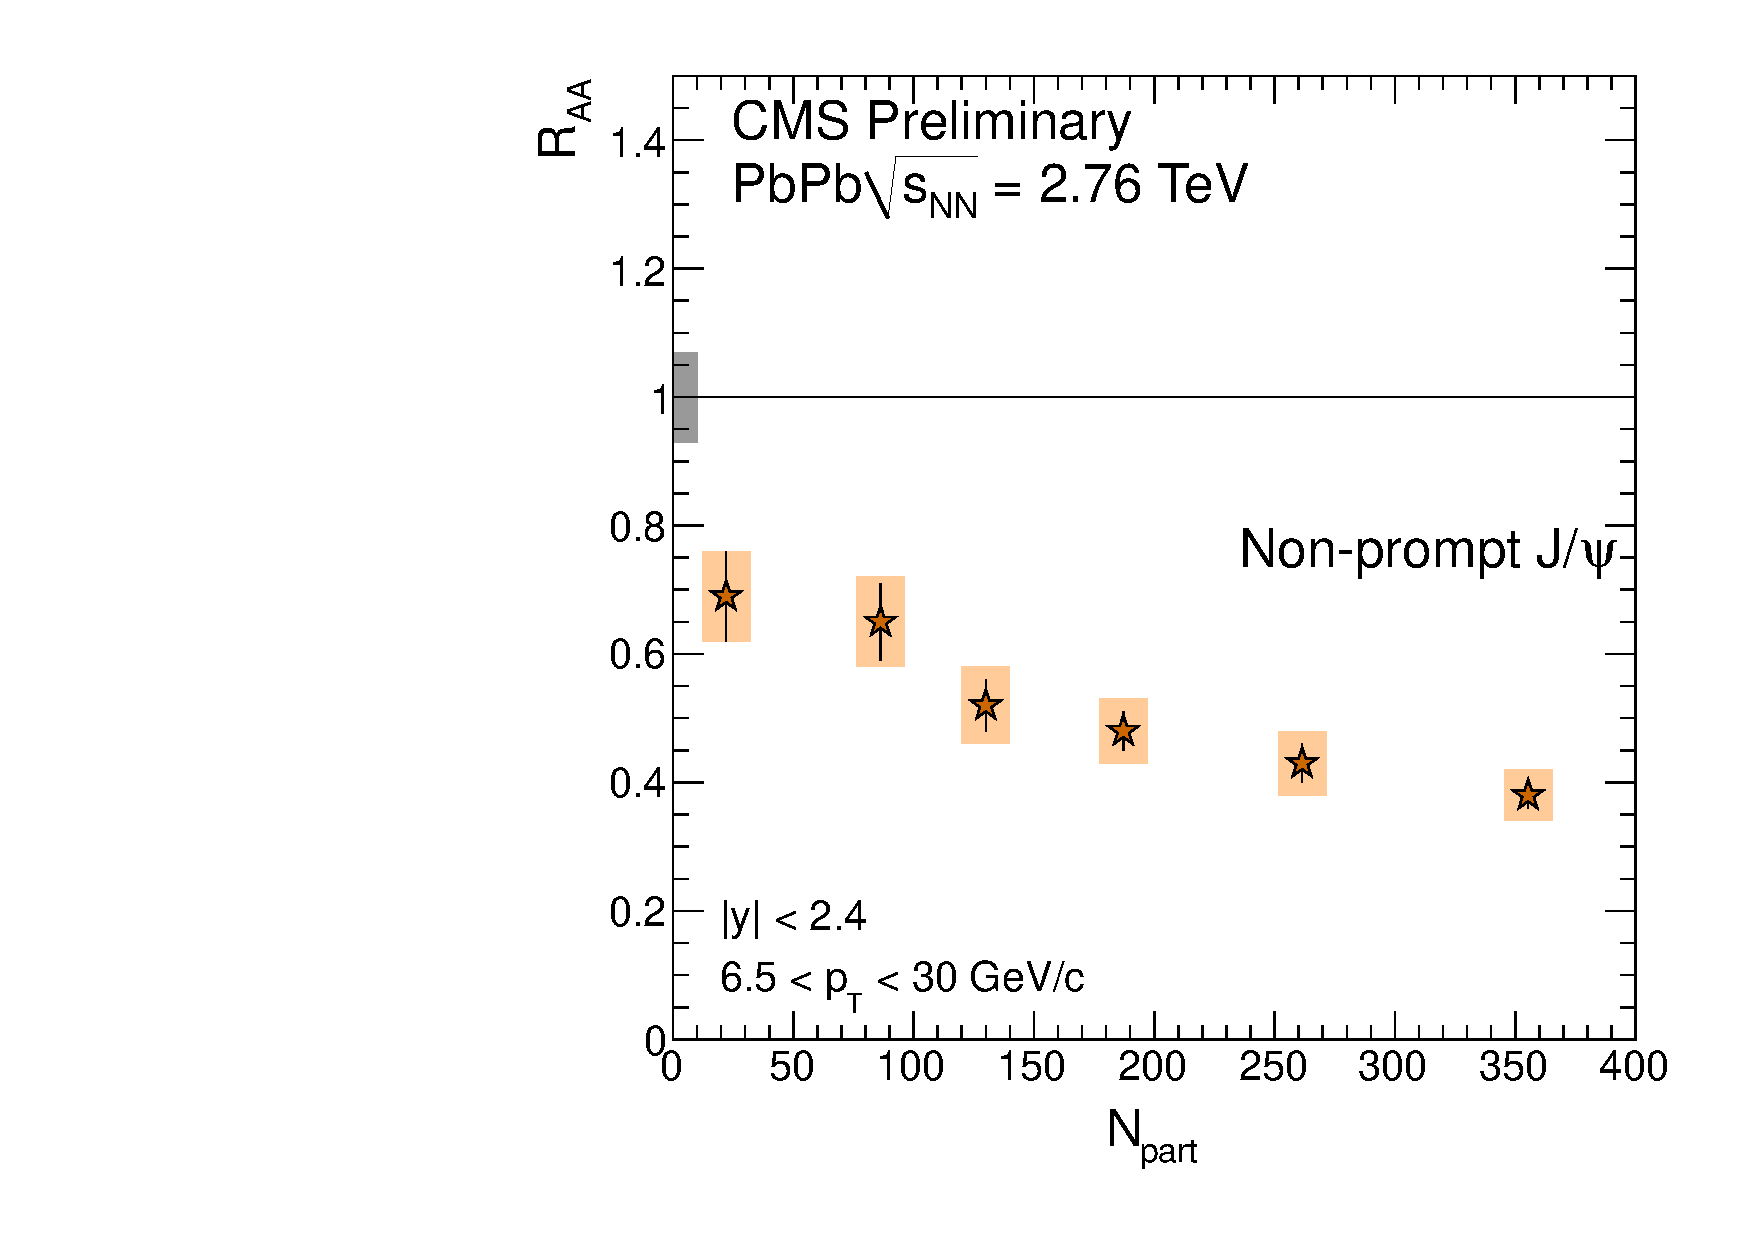
\includegraphics[width=0.7\textwidth]{Chapters/pQuarkonia/CMSNonPromptJpsi.pdf}
  \caption{high \pt \Jpsi suppression in PbPb collisions from CMS, as a function of
    the centrality of the collision. Top: prompt \Jpsi, Bottom:
    non-prompt \Jpsi. From~\cite{12014}.}
  \label{fig:CMSpsi}
\end{center}
\end{figure}



There may be nuclear
modification process(es) affecting the \Jpsi~production (pPb data from CMS~\cite{14009} and
ALICE~\cite{alicejpsipPb} that I have not covered here, and that seem to go in the direction
of a reduction of the \Jpsi~yield in cold nuclear matter). Finally, there is a lot of interest regarding the $\psi(2S)$
suppression in PbPb collisions. First, this is a very challenging measurement
given the naturally small $\psi(2S)$ yield when comparing with
\Jpsi. Second, a measurement from CMS~\cite{Khachatryan:2014bva} seems to show less suppression
for $\psi(2S)$ than for \Jpsi\ in an intermediate \pt\ region, where
some recombination effects could still be at play. This would only be
settled with a careful look at a more abundant PbPb dataset in the
coming years. In 2015, the LHC will operate Pb ion beams reaching an energy
in the center of mass of about 5 TeV, which will allow one to reach even
higher energy densities than previously, and will enhance slightly the
cross section for hard processes such as the \Jpsi\ and $\psi(2S)$.



% \vspace{0.5em}
% \begin{center}
%   \fbox{
%     \parbox{0.9\textwidth}
%     {\textsf { }}} 
% \end{center}

\clearpage
\section{The bottomonium case}

Since the $b$ quark mass is higher than the $c$ quark, it is likely that
perturbative calculations find a better agreement on \PgU~data than
what was observed in \Jpsi data. Also, one can make a more stringent test of the
non-relativistic hypothesis given the higher quark mass.
Although the feed-down fractions were known from \pt = 8 \GeVc and
above with Tevatron data, the LHC measurements provide with more
information on the transition from higher energy levels to the ground
state, which is an important constraint for our understanding of
\PgU~suppression in heavy ion collisions. The feed-down fractions from
\PgU(nS), $\chi_{b}$(mP), to \PgUa~were previously shown on
Figure~\ref{fig:bottomonium}.
\\
Next I will move to the case of bottomonia in heavy ions. The melting
temperature is expected to be different for states with different
binding, hence it is interesting to look for the yields of all three \PgU~states in
heavy ion collisions. These provide interesting constraints on the temperature of
the medium produced in heavy ion collisions at the energies of the LHC (as well
as RHIC energies as we shall see). In the case of \PgU~states, the
mass being larger than for charmonia, it is possible that binding
energies from potential models are more stable. When it comes to the nuclear
absorption effects and shadowing, these should also be smaller than
for charmonia, given the fact that the initial parton is slightly
harder. Finally I will present some results regarding \PgU\
measurements as a function of the event centrality in PbPb collisions
that exhibited a strong suppression of the excited states for the
first time, shortly before the beginning of my thesis.

\subsection{\texorpdfstring{\PgU}{Y} production in pp collisions}
The LHC data collected during Run 1 provides several useful
constraints on quarkonium production, and that is seen for \Jpsi
as well as for \PgU. We now turn to the case of \PgU~production in pp collisions.



The ATLAS experiment measures \PgU~states decaying in two muons in the
pseudorapidity range $\vert\eta^{\mu}\vert < 2.25$. %  (the branching
% fraction for \PgUa~to
% muons is $B_{\mu\mu} = 2.78 \%$).
This measurement in 7 TeV pp data~\cite{atlasUpsilon7tev} 
scans the \pt spectrum up to 70 \GeVc~with an integrated luminosity of $\lumi$ = 1.8 \invfb. The invariant mass plot for the central rapidities
$\vert y\vert <
1.2$ appears in Figure~\ref{fig:upsimass_pp} (top, left). 



CMS has measured \PgU~states in the dimuon channel with pp data at 7
TeV as well, dedicating two papers (post-ICHEP
2010 which consisted of about 3~\invpb~of 2010 data). The first
publication~\cite{cmsUpsi1} presented \PgU~spectra up to \pt = 50 \GeVc, with
approximately 36~\invpb~of pp data, using the full coverage of muon
detectors and of the inner tracking system, $\vert\eta\vert <
2.4$. Next, a further measurement~\cite{cmsUpsi2} using $\lumi$ = 4.9
\invfb of pp data focuses on events with $\pt > 10~\GeVc$ with a rapidity
cut at $\vert y^{\mu\mu}\vert < 1.2$, where the dimuon resolution is as good as
to separate clearly the three upsilon states, as shown in
Figure~\ref{fig:upsimass_pp} (top, right).

\begin{figure}[h]
\begin{center}
 \hspace{0.5cm} \includegraphics[height=0.2\textheight]{Chapters/pQuarkonia/AtlasUpsi.pdf}
  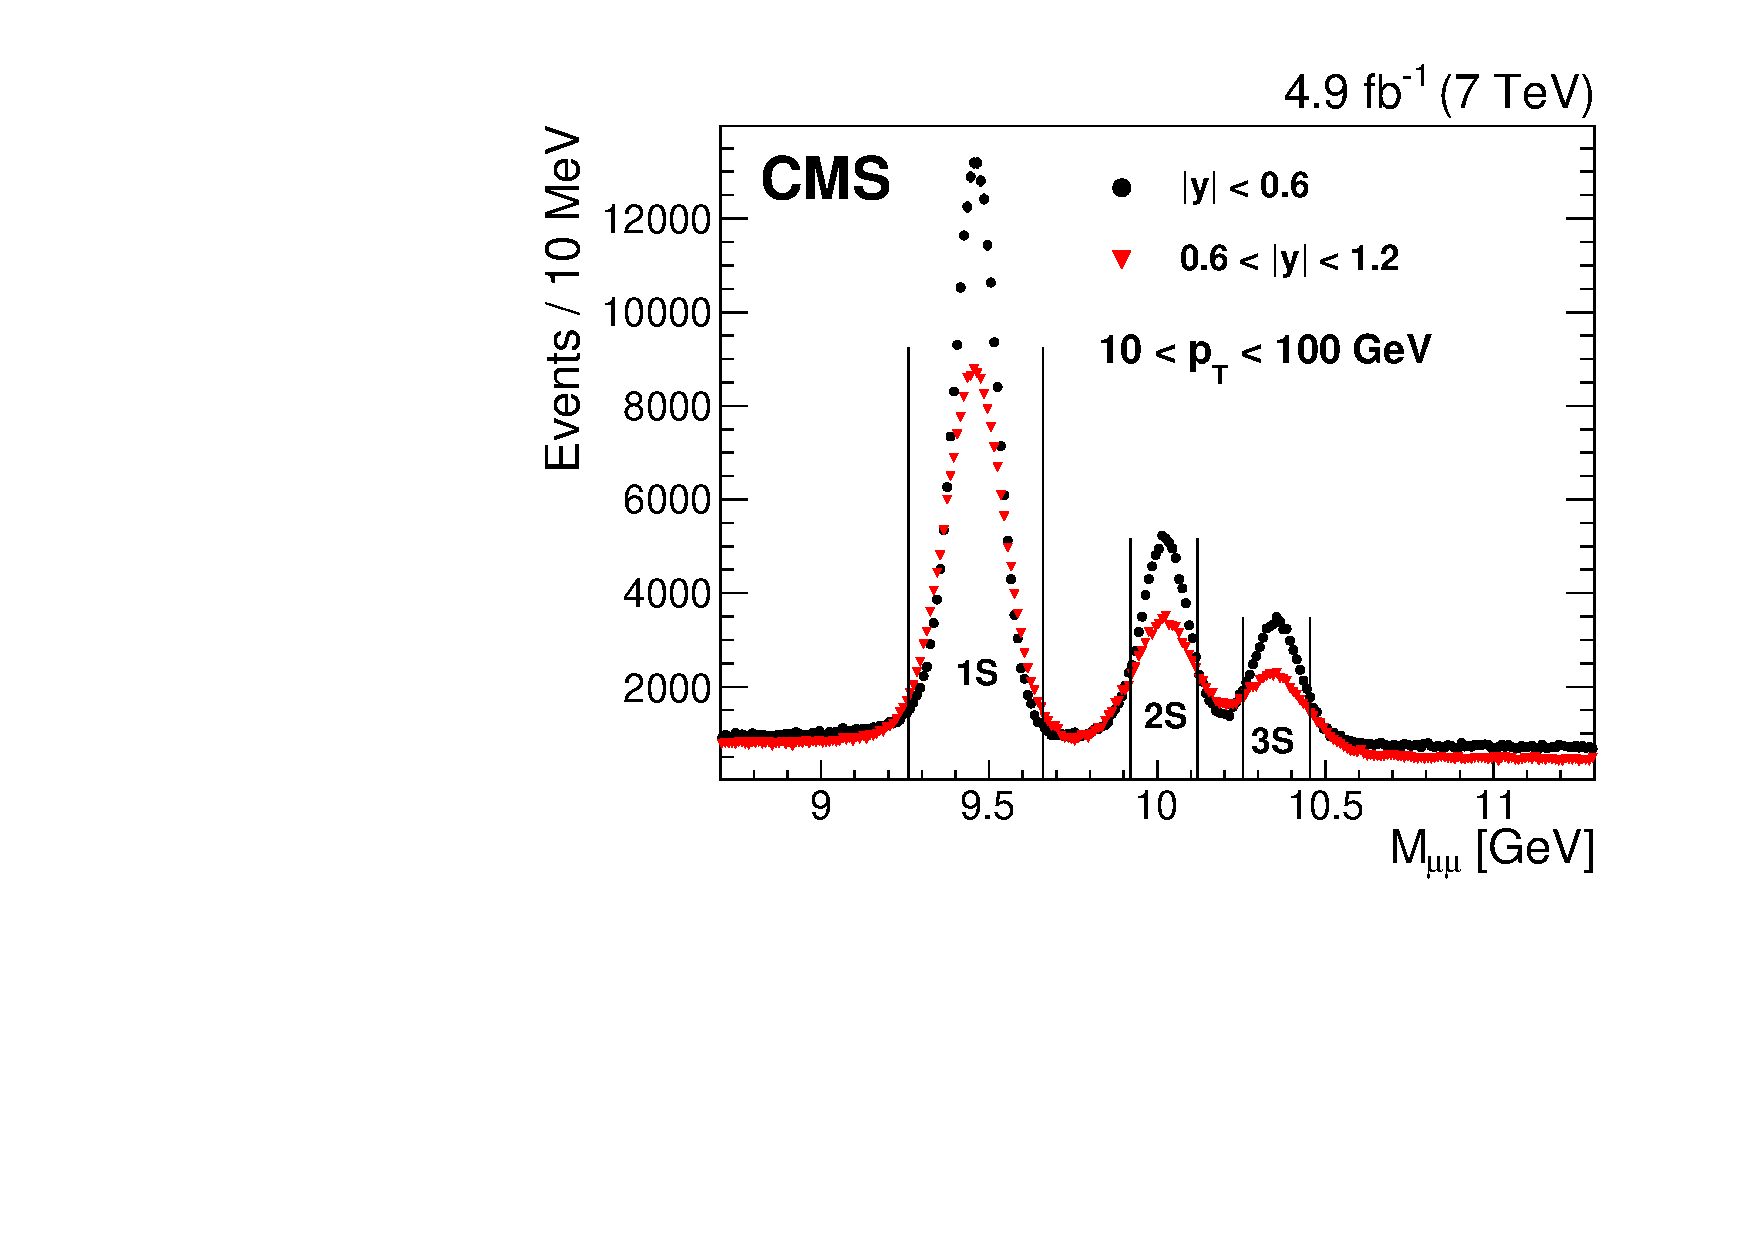
\includegraphics[height=0.21\textheight]{Chapters/pQuarkonia/CMSUpsi.pdf}
  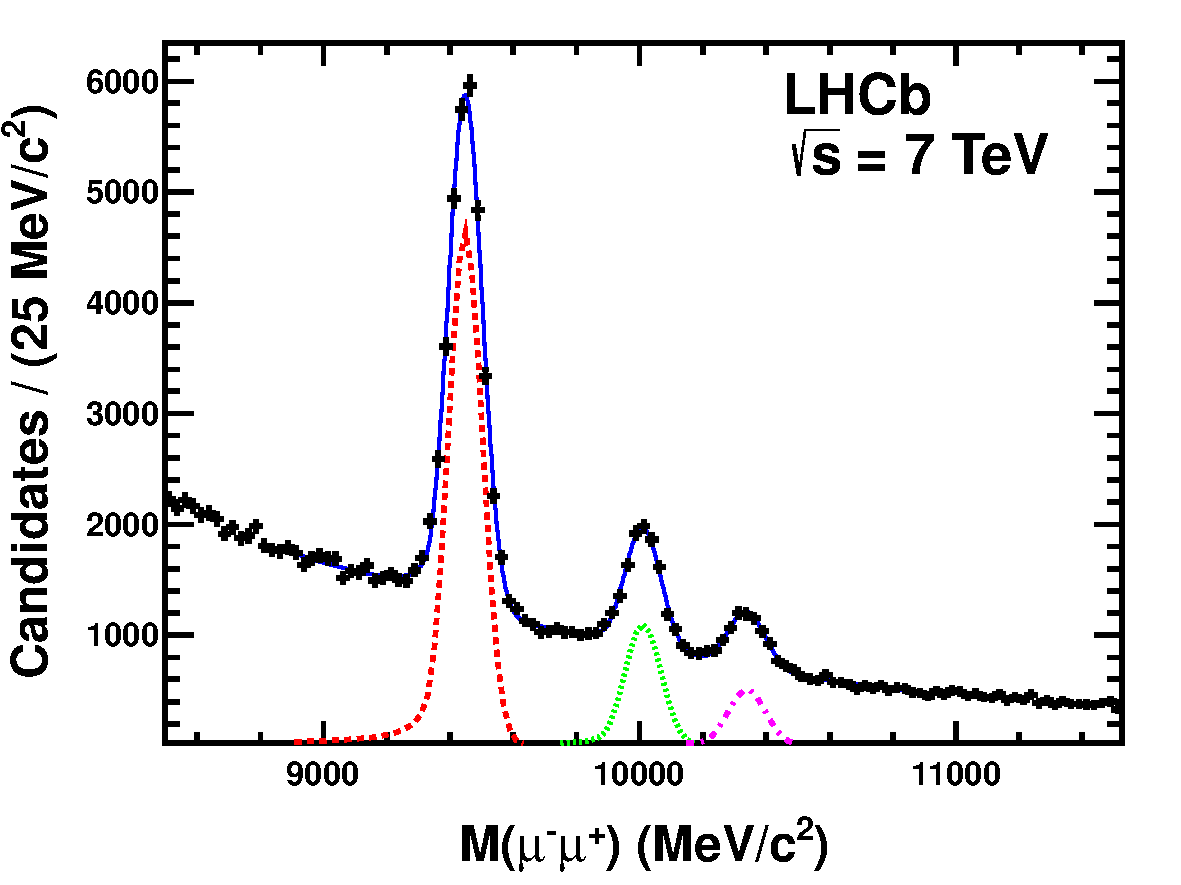
\includegraphics[height=0.21\textheight]{Chapters/pQuarkonia/lhcbUpsi.pdf}
  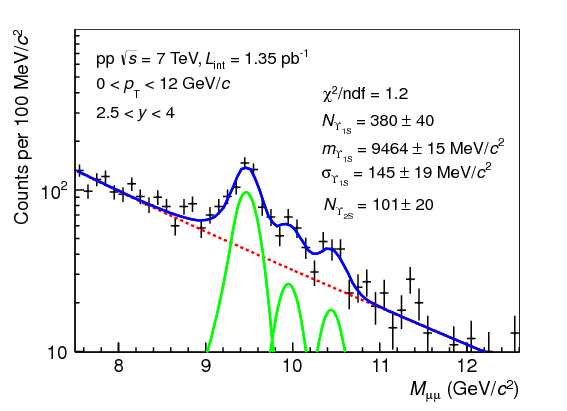
\includegraphics[height=0.21\textheight]{Chapters/pQuarkonia/AliceUpsi.png}
  \caption{The dimuon invariant mass distribution in the vicinity of
    the \PgU\ resonances for ATLAS data (top, left), CMS data (top,
    right), LHCb data (bottom left) and ALICE data (bottom right). The
    solid lines in ATLAS, LHCb and ALICE plots represent fits to the invariant mass distributions, as
  described in respective publications~\cite{atlasUpsilon7tev,lhcbUpsi1,aliceUpsi_pp}.}
  \label{fig:upsimass_pp}
\end{center}
\end{figure}


The LHCb collaboration has also measured \PgU~states in $\lumi = 36~\invpb$
of pp collisions at \s\ = 7 TeV, in a publication extending to events with $\pt < 15
\GeVc$, in the dimuon rapidity coverage of LHCb ($2.5 < y <
4$)~\cite{lhcbUpsi1}. The dimuon invariant mass plot in the \PgU~mass
range is presented in Figure~\ref{fig:upsimass_pp} (bottom, left).
%  A more recent LHCb paper~\cite{lhcbUpsi1fb} using
% \s\ = 7 TeV and \s\ = 8 TeV data has also been published, from which the
% \pt\ spectrum is displayed in Figure~\ref{fig:upsispectrapp}
% (bottom, left).


% but since the data set is not
% particularly larger than in~\cite{lhcbUpsi1} 7 TeV data, the
% comparison I am doing here relies on 7 TeV data only. Nevertheless one
% does not expect a lot of change between 7 TeV and 8 TeV quarkonium
% data, except a slightly higher cross section (as for other hard
% processes, the $Q\bar{Q}$ cross section increases with \s).



The ALICE collaboration has measured quarkonium states in 7 TeV
collisions as well, with $\lumi = 1.35 \invpb$ of pp data, recorded in the
rapidity range $2.5 < y < 4$. The measurement~\cite{aliceUpsi_pp} extends to \pt = 12
\GeVc, and the invariant mass plot is presented in
Figure~\ref{fig:upsimass_pp} (bottom, right).



The various mass plots of Figure~\ref{fig:upsimass_pp} are all
different in that they do not all span the same phase space window,
and the detector settings vary from one experiment to the other. The
unexhaustive details given here are based on the four plots of
Figure~\ref{fig:upsimass_pp}:
\begin{itemize}
\item[1.]{CMS and ATLAS invariant mass figures (upper panels of
    Figure~\ref{fig:upsimass_pp}) cover the mid-rapidity region,
    $\vert y \vert < 1.2$. The analyses performed in the two experiments are
    comparable, in terms of reconstruction and trigger strategies. As
    a consequence, the only difference comes from the mass resolution
    of the peaks: in ATLAS, the reported $\Upsilon(1S)$ width is 120
    MeV, while in CMS it is roughly two times less (the actual number
    for the presented plot was not made public). The broader peak seen
    in ATLAS is explained by the smaller magnetic field intensity,
    rendering a poorer momentum resolution on individual muons. The
    momentum resolution in both experiments is of the order of 1 to 5
    \% for \Jpsi\ muons, as reported in~\cite{Aad:2014rra,CMS:2010oua}.}
\item[2.]{ALICE and LHCb have similar rapidity coverage, $2.5 < y <
    4$, a region where the dimuon mass spectrum can
    be populated with combinatorial background exponentially
    decreasing with increasing dimuon mass, as is seen in both figures
    (lower panels of
    Figure~\ref{fig:upsimass_pp}).}
\end{itemize}


The \pt spectra are measured in all four experiments, and presented
in Figure~\ref{fig:upsispectrapp}. The differential cross sections are
computed after extracting the yield from invariant mass plots similar to what is
shown on Figure~\ref{fig:upsimass_pp}, with a differential binning in
the observable under consideration, \pt\ or \y. The extraction is performed using
empirical functions to describe the signal and background, which are
fitted to data. For each peak, as is shown in
Figure~\ref{fig:upsimass_pp} (top, left and bottom, right) there is a
different fit curve, and each curve is integrated to get a raw
yield for the considered \PgU~state. The yield is further corrected
for effects relative to the detectors inefficiencies or inadequate
modeling. Applying the proper luminosity normalisations and efficiency
corrections, one can derive a differential cross section times
branching fraction for the signal observed in the dimuon channel (as
it would be the case in our analysis).
\\
\begin{figure}[h]
\begin{center}
 \hspace{0.5cm} 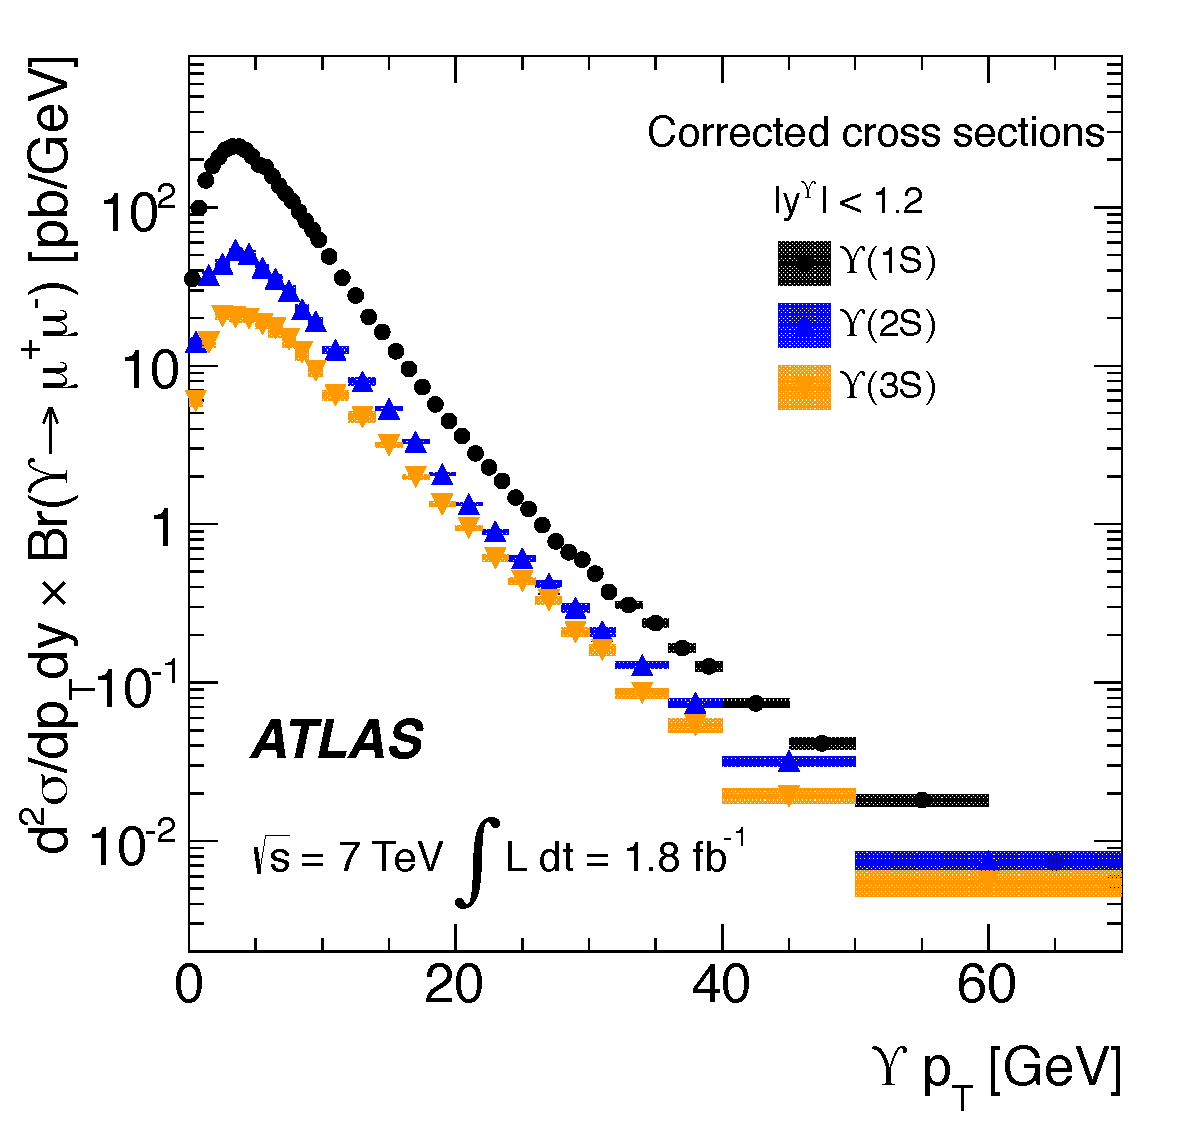
\includegraphics[height=0.25\textheight]{Chapters/pQuarkonia/AtlasUpsiPtNude.pdf}
  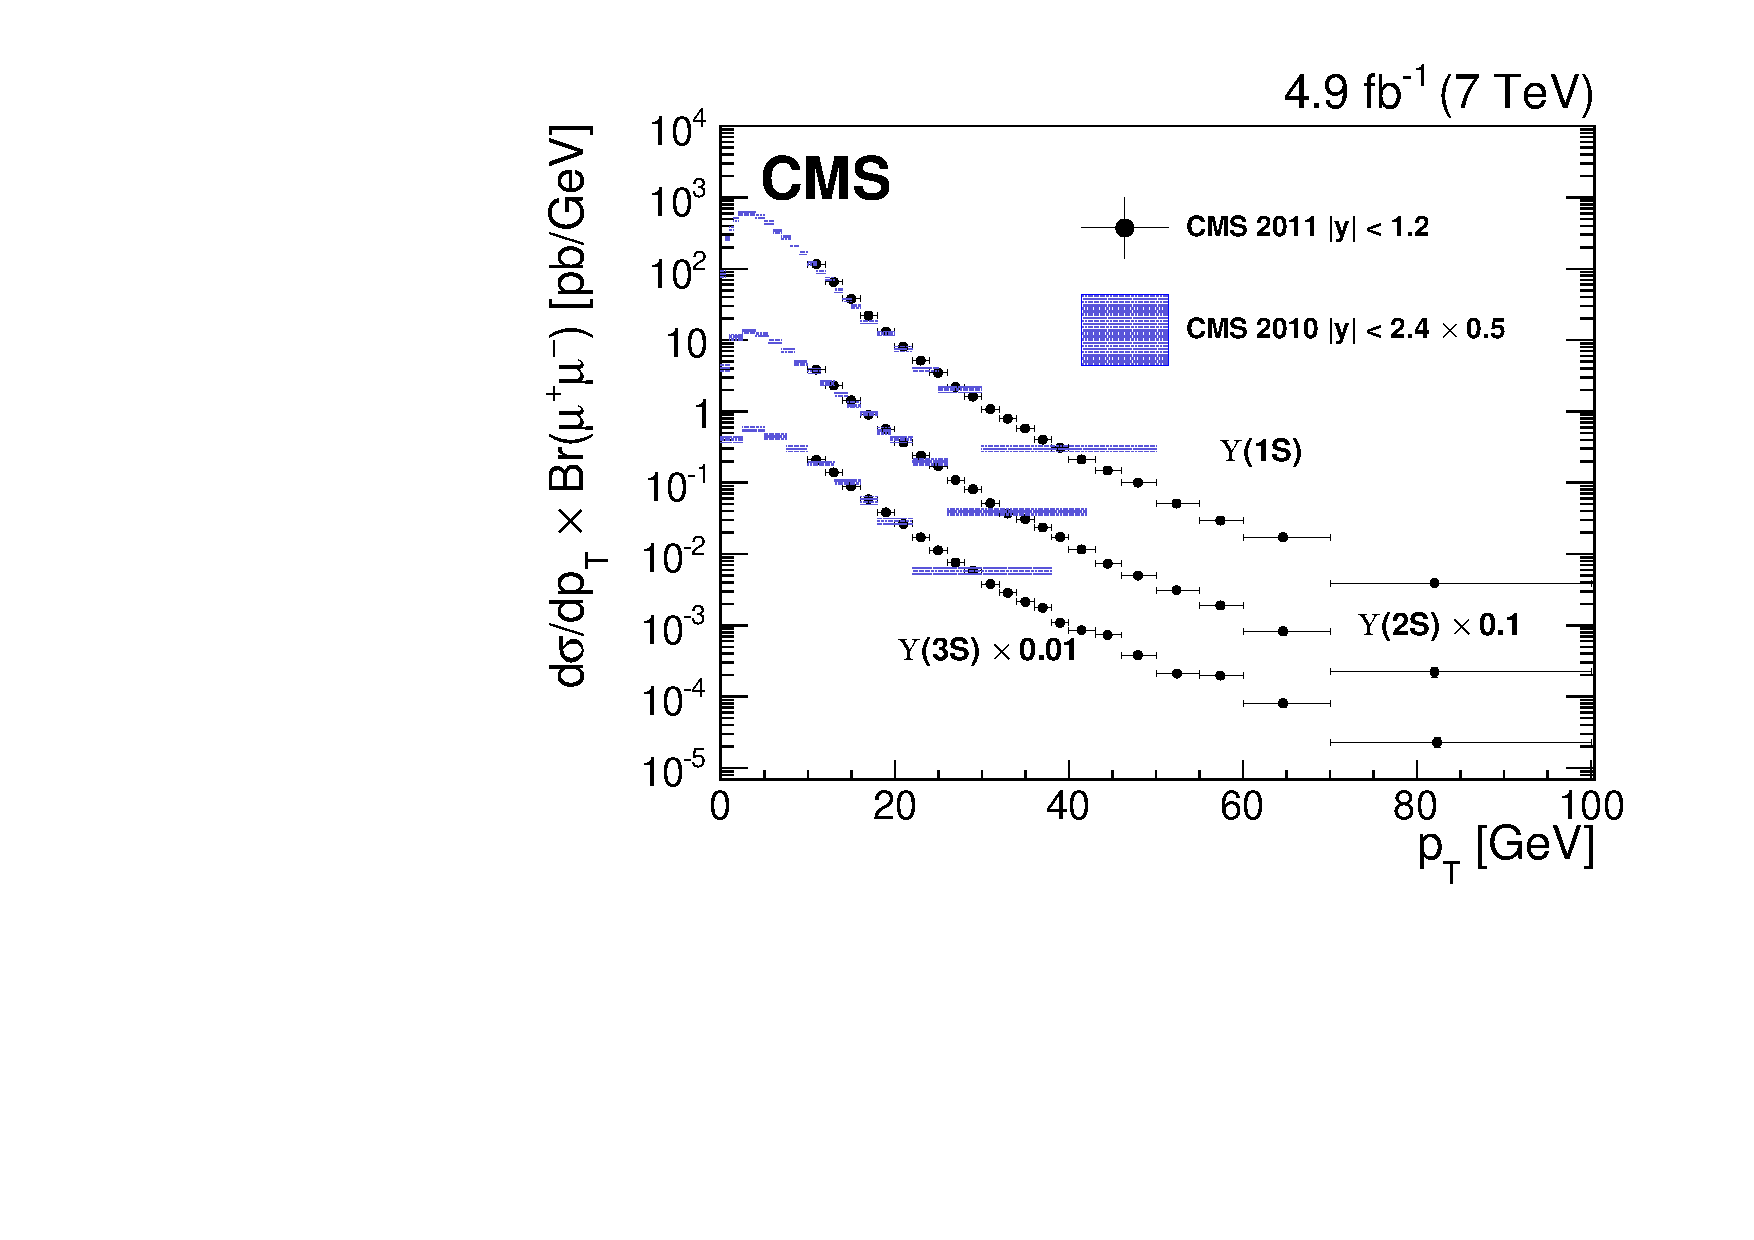
\includegraphics[height=0.25\textheight]{Chapters/pQuarkonia/CMSUpsiPt.pdf}
  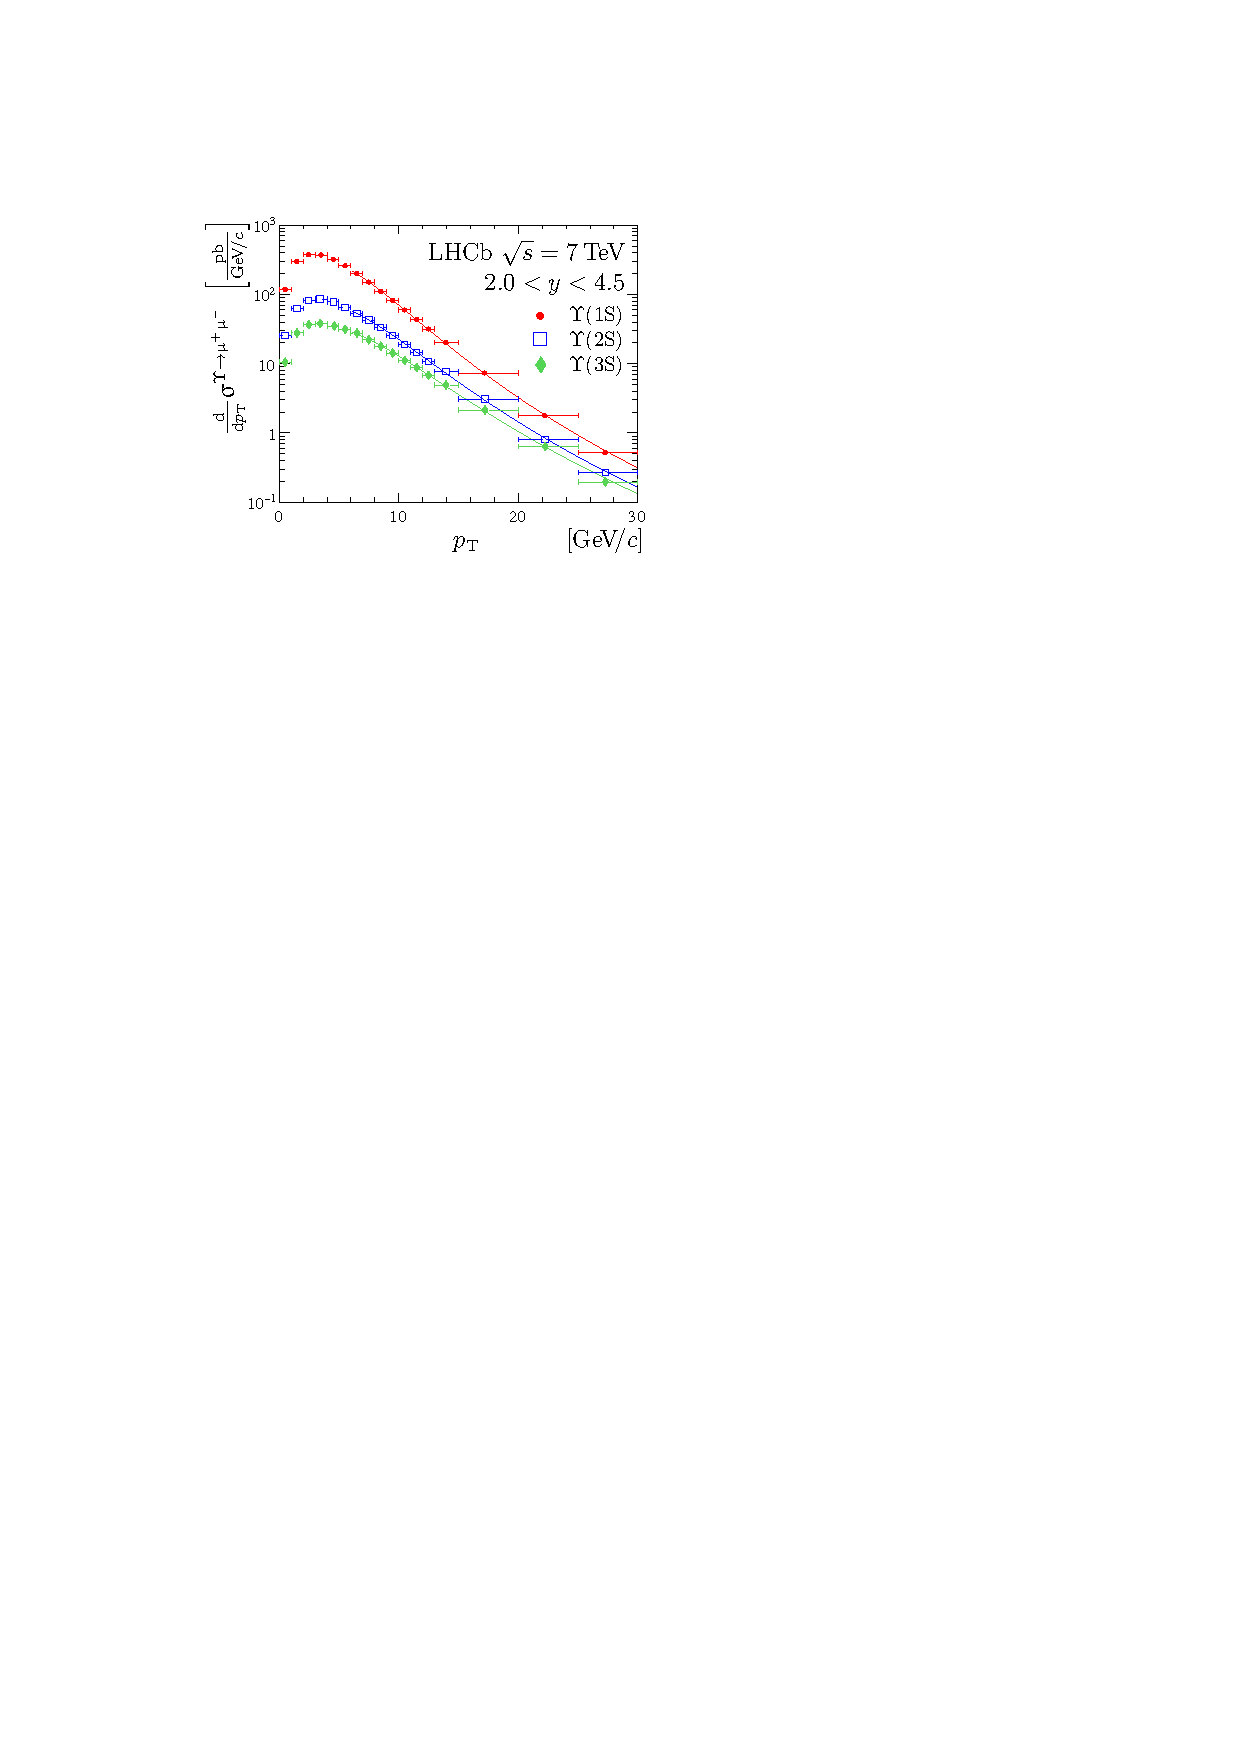
\includegraphics[height=0.25\textheight]{Chapters/pQuarkonia/lhcbUpsiPtTsallis.pdf}
  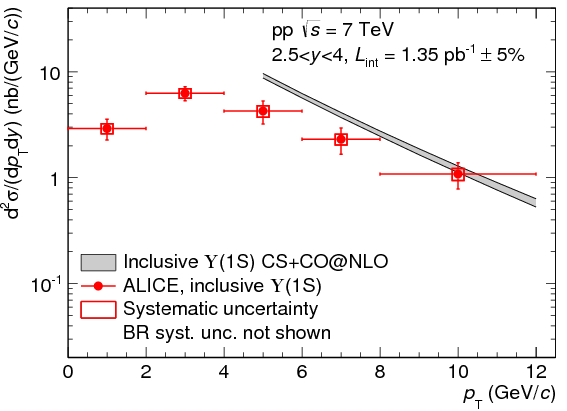
\includegraphics[height=0.23\textheight]{Chapters/pQuarkonia/AliceUpsiPtCSCONLO.png}
  \caption{Transverse momentum dependence of \PgU~states' production
    in pp data at 7 TeV. Data from ATLAS (top, left)~\cite{atlasUpsilon7tev}, CMS (top,
    right)~\cite{cmsUpsi1},~\cite{cmsUpsi2}, LHCb (bottom left)~\cite{lhcbUpsi1fb}, and ALICE (bottom right)~\cite{aliceUpsi_pp}. The
    CMS data displayed also contains low-\pt results from a 2010
    analysis~\cite{cmsUpsi1}, scaled to account for the
    rapidity range difference with~\cite{cmsUpsi2}. The LHCb data is
    fitted with a Tsallis distribution function as described
    in~\cite{lhcbUpsi1fb}. The ALICE data is compared to a NLO
    prediction of quarkonium production in the NRQCD approach~\cite{nrqcdupsilon}.}
  \label{fig:upsispectrapp}
\end{center}
\end{figure}



After having applied all corrections that give a proper image of the
physical rate of \PgU~production in the experiment, one can compare to
theoretical models, such as the ones presented in Section~\ref{sec:models}.
With their larger mass, the perturbative calculations in QCD are
expected to yield more accurate results on bottomonia than what we have seen previously
for \Jpsi. 

Figure~\ref{fig:atlasNNLO} shows a theory comparison of ATLAS \PgUa~cross section results to the CSM
expectation, scaled to a normalisation factor, and the
CSM calculation is taken up to some terms of the
$\mathcal{O}(\alpha_{S}^{5})$ expansion, that is,
at partial next-to-next-to-leading order
(NNLO$^{\star}$)~\cite{LansbergNNLO}. The star symbol is 
here to indicate that the only NNLO terms considered in this
calculation are those considered by the author of~\cite{LansbergNNLO}
to give a dominant contribution in the $\alpha_{S}^{5}$. As is shown
in the first
bottom panel of the figure, the NNLO$^{\star}$ prediction drops faster
than the data at high \pt. Another
comparison visible in the lowest panel of Figure~\ref{fig:atlasNNLO}
is the CEM expectation, and this one shows another disagreement, again
with large uncertainties. The blue band associated with data points
results from a variation of polarisation hypotheses. Spin
alignment measurements have been since performed, for example with CMS
$\Upsilon$ data, for which the result will be presented below.
\\
\begin{figure}
\begin{center}
  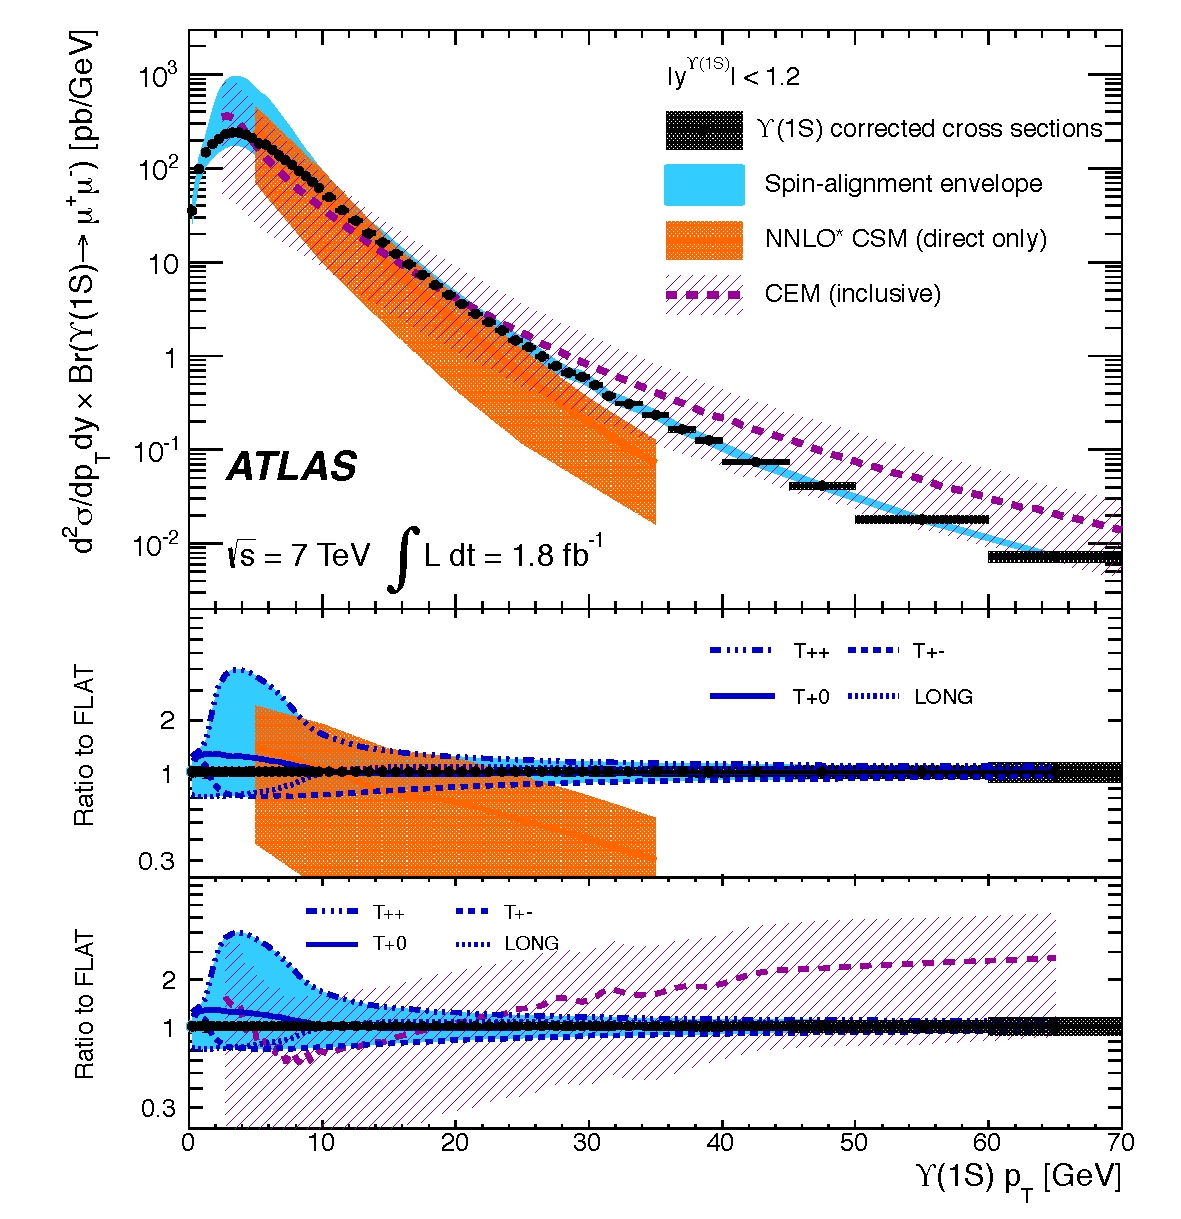
\includegraphics[height=0.4\textheight]{Chapters/pQuarkonia/AtlasUpsiPt.pdf}
  \caption{\PgUa~differential cross section as a function of \pt, from
    ATLAS 7 TeV pp data~\cite{atlasUpsilon7tev}. Model comparisons
    include a truncated $\mathcal{O}(\alpha_{S}^{5})$ calculation
    (NNLO$^{\star}$) from the colour singlet model (CSM), in an orange
    uncertainty band, compared to data in the intermediate panel. The
    bottom panel has a colour evaporation model (CEM) prediction compared to
    data. On all panels, the blue band corresponds to a variation of
    the acceptance corrections with maximal longitudinal and transverse polarisations.}
  \label{fig:atlasNNLO}
\end{center}
\end{figure}



The ALICE \PgUa~\pt~spectrum in Figure~\ref{fig:upsispectrapp} shows a
comparison with NRQCD (that is, including colour singlet and
colour octet contributions) at NLO, which seems to find quantitative agreement
at high \pt. As mentioned in Section~\ref{sec:models}, one should note that NRQCD developments~% (which
% are usually done over the whole phase space, contrary to what is
% displayed here) 
predict a large transverse polarisation for \Jpsi or \PgU\ resonances, saturating
to an almost full transverse polarisation at high \pt. One should then
compare NRQCD expectations to the polarisation of measured quarkonia
in hadron-hadron collisions to look for a possible agreement.



CMS has published a measurement of the polarisation of all three
\PgU(1S,2S,3S) states in pp collisions in~\cite{CMSupsipol}. The
results for \PgUa\ and \PgUc\ are displayed in Figure~\ref{fig:upsipol}. It shows a helicity component $\lambda_{\vartheta}$ compatible with
zero for both \PgUa\ and \PgUc, and is overlayed with a theory
comparison in the case of~\PgUc. As one can see, in the NRQCD
formalism and contrary to the CSM, colour octet and higher order
contributions should exhibit a transverse polarisation for S-wave
quarkonia. Unfortunately, the agreement seen in \pt spectra
(relatively good, given uncertainty bands) should be taken with
caution because of this.
\begin{figure}[h]
\begin{center}
  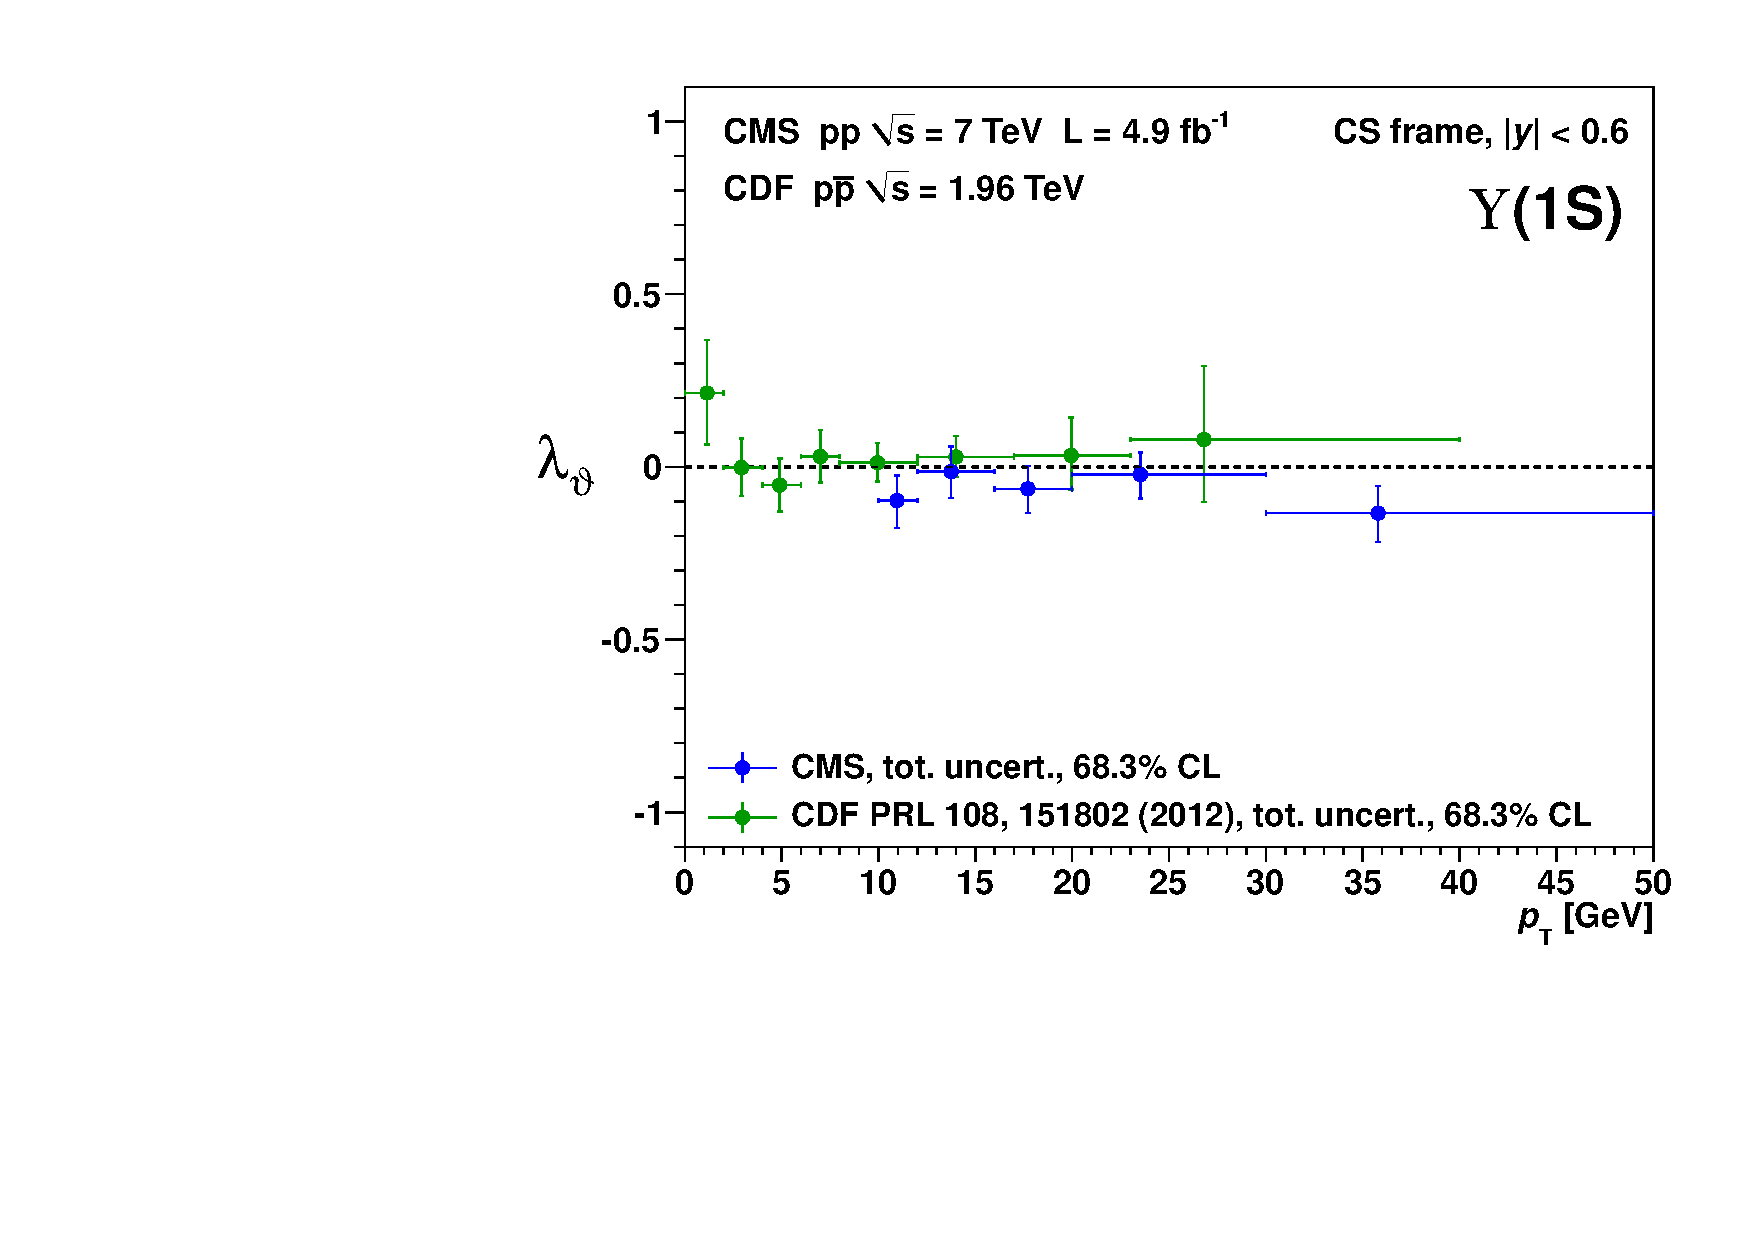
\includegraphics[height=0.25\textheight]{Chapters/pQuarkonia/cmscdfupsipol1.pdf}
  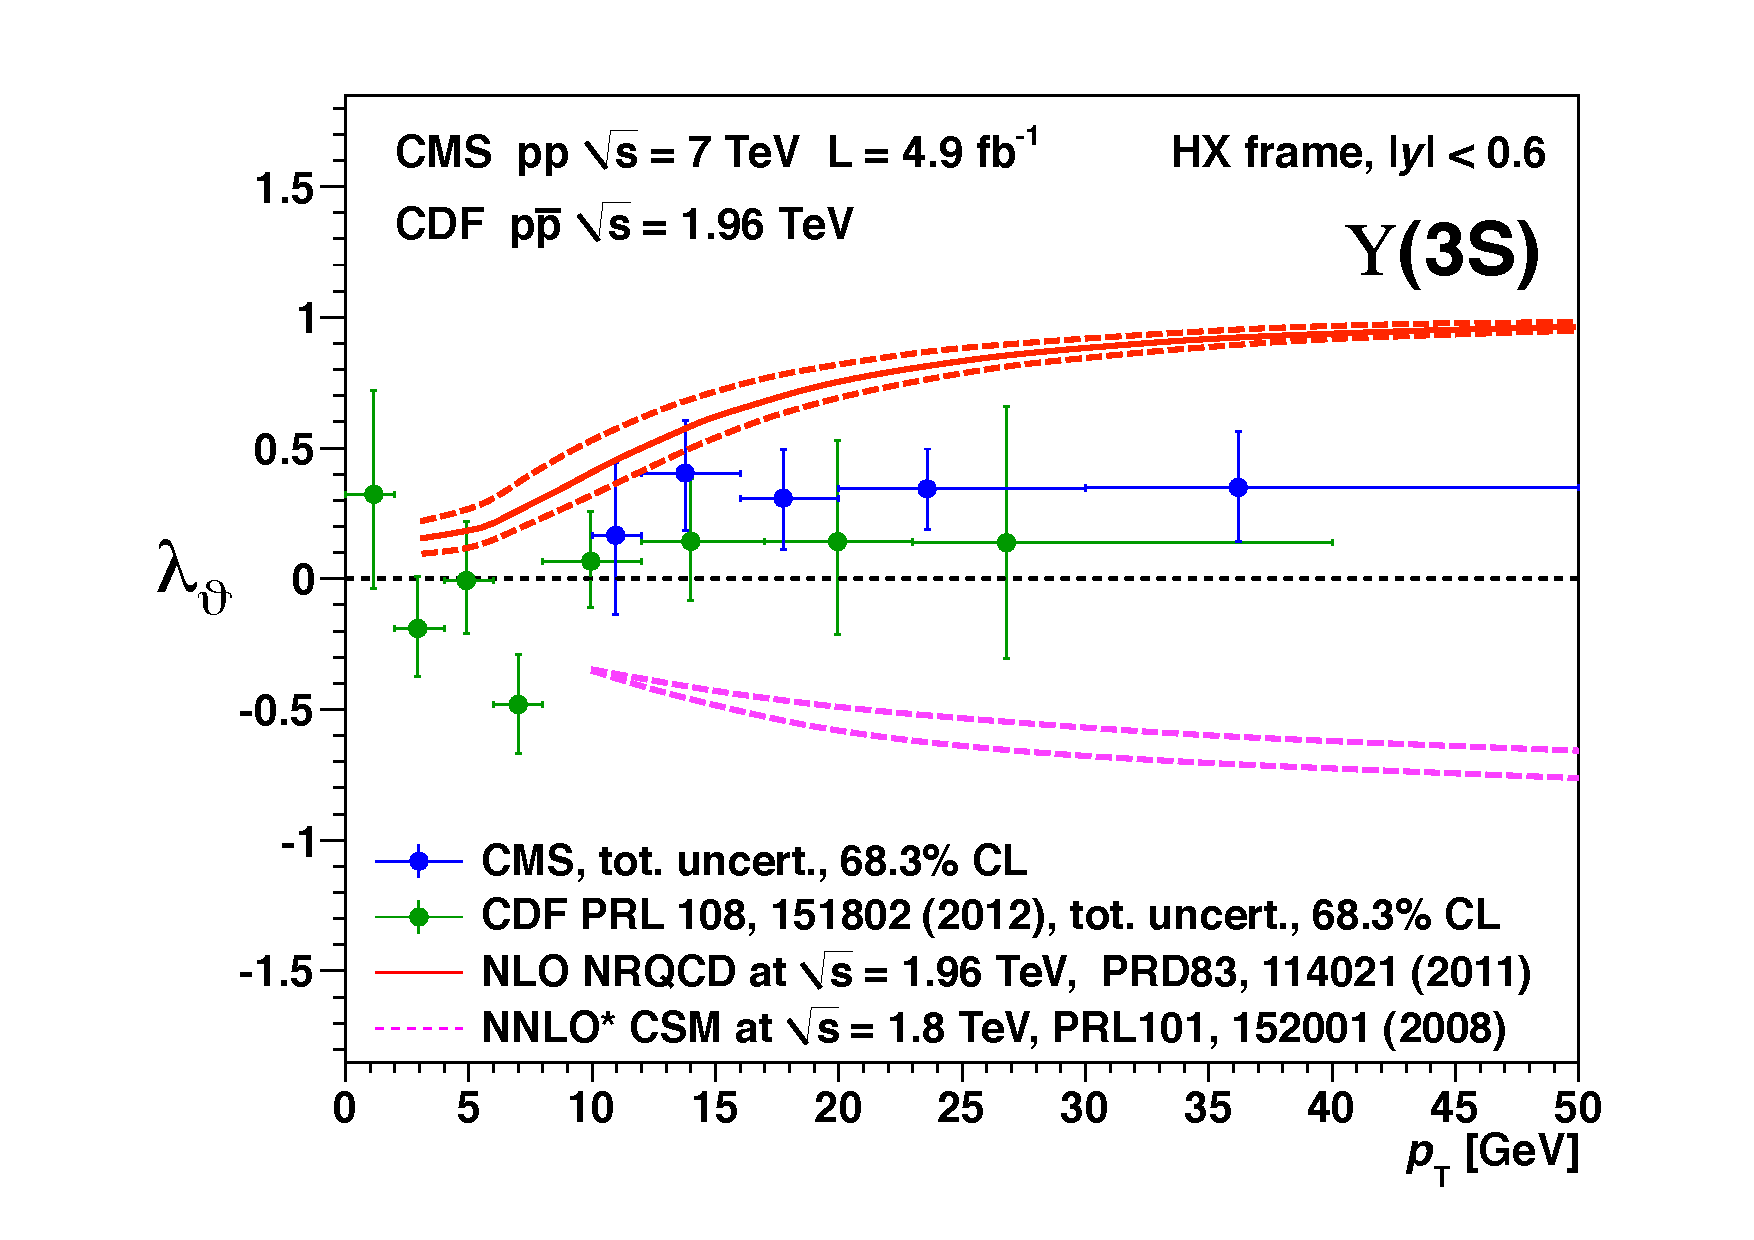
\includegraphics[height=0.25\textheight]{Chapters/pQuarkonia/CMSCDFupsipol3.pdf}
  \caption{\PgUa~and \PgUc~polarisations measured by CMS in $pp$ and
    compared to CDF (Tevatron) in $p\bar{p}$ collisions as a function
    of \pt. The vertical axis corresponds to 
    the polarisation component in the helicity frame (HX). Taken from~\cite{CMSupsipol}.}
  \label{fig:upsipol}
\end{center}
\end{figure}
To elaborate more on comparisons with NRQCD without going into polarisation details
(which may be poorly constrained when the prediction is restricted to a
phase space region), I would like to end with a comparison of LHCb
cross section data from~\cite{lhcbUpsi1fb} for \PgU(1S,2S,3S) versus
\pt and rapidity. Figure~\ref{fig:crosssectionratiolhcb} shows the
ratio of such cross sections at the two \s\ = 7 and 8
TeV energies, $\mathcal{R}_{8,7} = \sigma(\Upsilon(nS))_{\s = 8\textrm{TeV}}/\sigma(\Upsilon(nS))_{\s = 7\textrm{TeV}}$. NRQCD predicts a large contribution of the CO terms
in the cross section ratio, the colour singlet contributions mostly
canceling as is emphasised in~\cite{lhcbUpsi1fb}. The prediction for
the cross section ratio in NRQCD does in fact depend sharply on rapidity and is
plotted in straight lines in Figure~\ref{fig:crosssectionratiolhcb} (black on the left for the \pt-dependence,
coloured on the right for the rapidity dependence). This disagreement
in the comparison of the \s\ evolution of NRQCD predictions to data is
a striking feature of our lack of theoretical modeling of quarkonia in hadroproduction.



\begin{figure}[h]
\begin{center}
  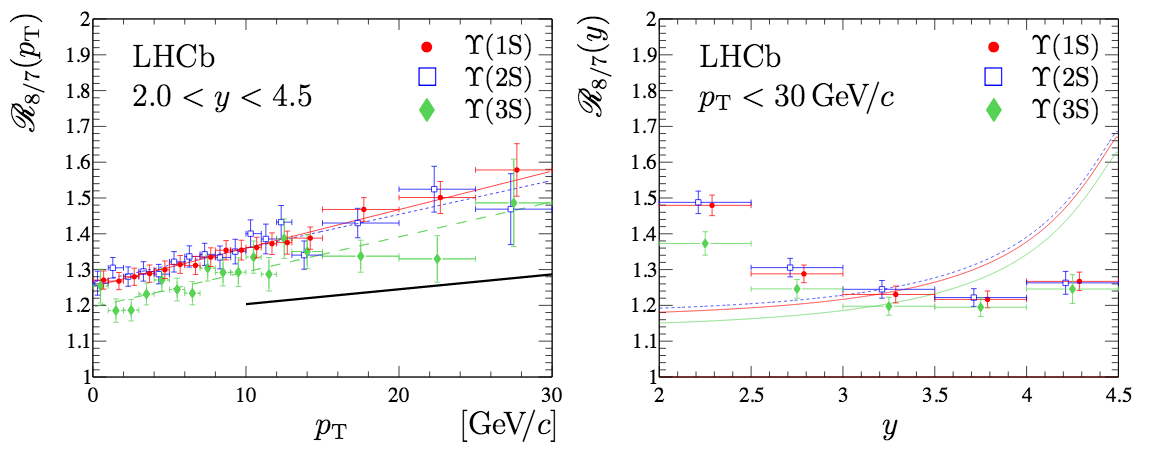
\includegraphics[height=0.25\textheight]{Chapters/pQuarkonia/lhcbUpsiRapidityRatio.png}
  \caption{Ratio of \PgU~ cross sections as a function of rapidity for
    two different centre-of-mass energies, \s\ = 7, 8 TeV, from
    LHCb. On the left, the black line represents the \pt-dependent
    expectation from NRQCD. To the right, the prediction is dependent
    on the level of the state, and each line corresponds to the NRQCD
    prediction for its state (red: \PgUa, blue: \PgUb, green: \PgUc). Taken from~\cite{lhcbUpsi1fb}.}
  \label{fig:crosssectionratiolhcb}
\end{center}
\end{figure}


In order to complete our picture of the bottomonium family, we must take some
time to analyse the other states with some detail:
the $\chi_{b}$ mesons and their decay are important to understand the
production rates for bottomonia in general, as these states are
usually quite difficult to detect as we shall see. The $\chi_{b}$
mesons are pseudovectors (even parity) and correspond to the following
spectroscopy levels~\cite{Agashe:2014kda}~\cite{chib3p_lhcb}:
\begin{eqnarray*}
\chi_{bJ}(mP) \Longrightarrow  m = \textrm{energy level},\: j &=&
\textrm{value of angular momentum J as in }J^{PC};\\
m(\chi_{b0}(1P)) &=& 9859.44 \pm 0.42 \pm 0.31\: \MeV\\
m(\chi_{b1}(1P)) &=& 9892.78 \pm 0.26 \pm 0.31\: \MeV\\
m(\chi_{b2}(1P)) &=& 9912.21 \pm 0.26 \pm 0.31\: \MeV\\
&--&\\
m(\chi_{b0}(2P)) &=& 10\,232 \pm 0.40 \pm 0.50\: \MeV\\
m(\chi_{b1}(2P)) &=& 10\,255 \pm 0.22 \pm 0.50\: \MeV\\
m(\chi_{b2}(2P)) &=& 10\,268 \pm 0.22 \pm 0.50\: \MeV\\
&--&\\
m(\chi_{b0}(3P)) &=& ??\: \MeV\\
m(\chi_{b1}(3P)) &=& 10\,511 \pm 1.7 \pm 2.5\: \MeV\\
m(\chi_{b2}(3P)) &=& 10\,551 \pm 14 \pm 17\: \MeV\\
\end{eqnarray*}
\\
These states are all important in the bottomonium spectroscopy as some
account for up to 30 \% of one of the (S-wave) \PgU~yields. They are
especially hard to detect in hadron-hadron collisions, because their
favorite decay (apart from the many-gluon channel, which is intangible) is
$\chi_{b} \to \Upsilon + \gamma$, and the photon often carries a quite
small momentum (of the order of 500 \MeV), making it difficult to
detect. The photons can be reconstructed by their $e^{+}e^{-}$
conversion in the tracker or the electromagnetic calorimeter of most
LHC experiments, but because of the small photon momentum, the probability
for reconstructing this decay is \textit{very} small (of the order of
less than a percent, at low-\pt, in CMS).
\\
Fortunately, the fractions of $\chi_{b}$ mesons decaying to
\PgU~states, either via emission of a $\rho$ meson or two pions, or a
photon, can be well reconstructed at moderate-\pt, especially by
LHCb, which performed a first-time measurement of
the $\chi_{b1}(3P)$ mass and feed-down fraction towards \PgUa, \PgUb\
and \PgUc~\cite{chib3p_lhcb}.


These feed-down fractions are especially important in the
understanding of two (quite orthogonal) points in bottomonium physics:
first of all, the polarization and production rates of most
lower-lying states in theoretical models, such as \PgUc, which rely a
lot on the (expectedly small) fraction coming from
$\chi_{bJ}(3P)$. Second, the intepretations of \PgUa~suppression in heavy ions (pA or
AA) are strongly dependent on what is expected for the $\chi_{bJ}(1P)$
states, which are quite well measured in $pp$ and $e^{+}e^{-}$
collisions, but are still elusive in heavy ion experiments. The
feed-down fractions go as high as 30\% at high \pt, with a clear
\pt~dependence as is shown in Figure~\ref{fig:feeddown_lhcb}~\cite{chib3p_lhcb} in the case of $\chi_{b}(mP) \to \PgUa$
decays through a dipolar E1 transition. 


\begin{figure}
\begin{center}
  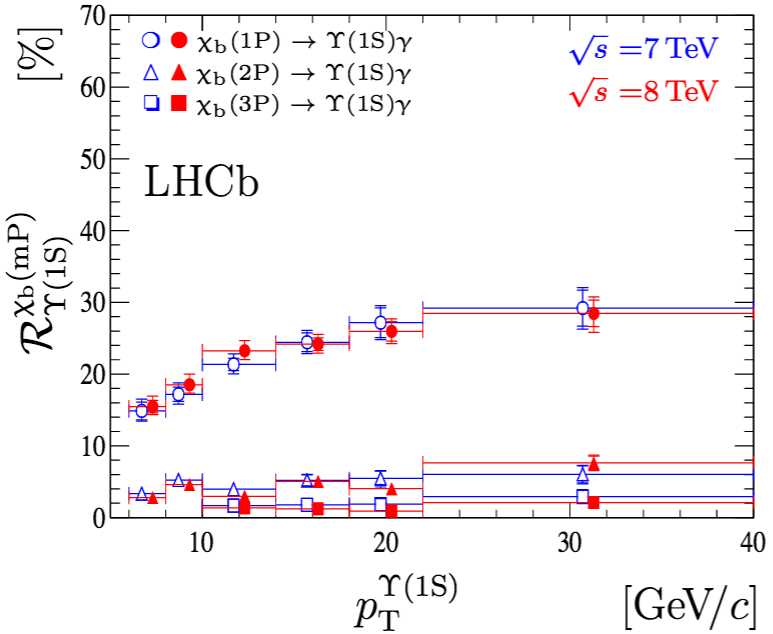
\includegraphics[height=0.35\textheight]{Chapters/pQuarkonia/chibfeeddown.png}
  \caption{Measurements of the feed-down fractions of $\chi_{bJ}(mP)$
    states to \PgUa~at LHCb. From~\cite{chib3p_lhcb}.}
  \label{fig:feeddown_lhcb}
\end{center}
\end{figure}



\subsection{\texorpdfstring{\PgU}{Y} suppression in heavy-ion
  collisions}

After the review on \PgU~production, which was aiming at a proper
'calibration' of the $pp$ reference measurement, I now turn to the
measurements of \PgU~mesons in heavy ion collisions.
\\
First of all, it may be worth noting that bottomonia in general, when
compared to charmonia, represent cleaner probes of the QGP. In the case of charmonium states, newer
measurements have often (if not always) led to more complicated
interpretations related to the relatively small mass of the
quark-antiquark pair. Even if the mass of charm quark is quite
large ($m_{c} \sim 1.5~\unitMass$) compared to light quark masses $m_{d},
m_{u}, m_{s}$ and to $\Lambda_{QCD}$, the measurements at the SPS
followed by RHIC and the LHC could not bring a unifying physical
interpretation of the nuclear matter effects on charmonia.



%  Then RHIC measurements came
% along, and with their clear suppression, a deconfinement effect was
% clear, although the increased suppression in the forward direction was
% interpreted either as a nuclear shadowing or absorption
% effect. Additionally, one can suggest that the lesser suppression at
% RHIC in the central rapidity region is a precursor of a recombination
% effect, although the \pt-dependence of the nuclear modification factor
% seems to tell otherwise.




% Finally, LHC measurements of charmonium suppression see a clear
% suppression in all cases, which can be largely enhanced at low-\pt,
% as the ALICE collaboration sees in the central rapidity region and in
% high centrality classes, favoring the statistical recombination
% picture (the recombined charm quark cross section being higher with
% high multiplicities and at $y \sim 0$). Also, the decreasing PbPb yield at
% forward rapidities can be seen as either a reduction of the
% recombination fraction with high rapidities, or a nuclear absorption
% effect. And this is particularly problematic in the sense that it
% depends to whom one asks. All these effects can be sizable for \Jpsi,
% but it is not clear what the fate of $\psi(2S)$ mesons would be, and
% the recent measurement of CMS~\cite{2Storsten} also goes in the
% direction of less suppression in the low-\pt, forward rapidity, very
% central rapidity region of the heavy ion collision phase space,
% without being conclusive.
% \\
\begin{figure}[t]
\begin{center}
  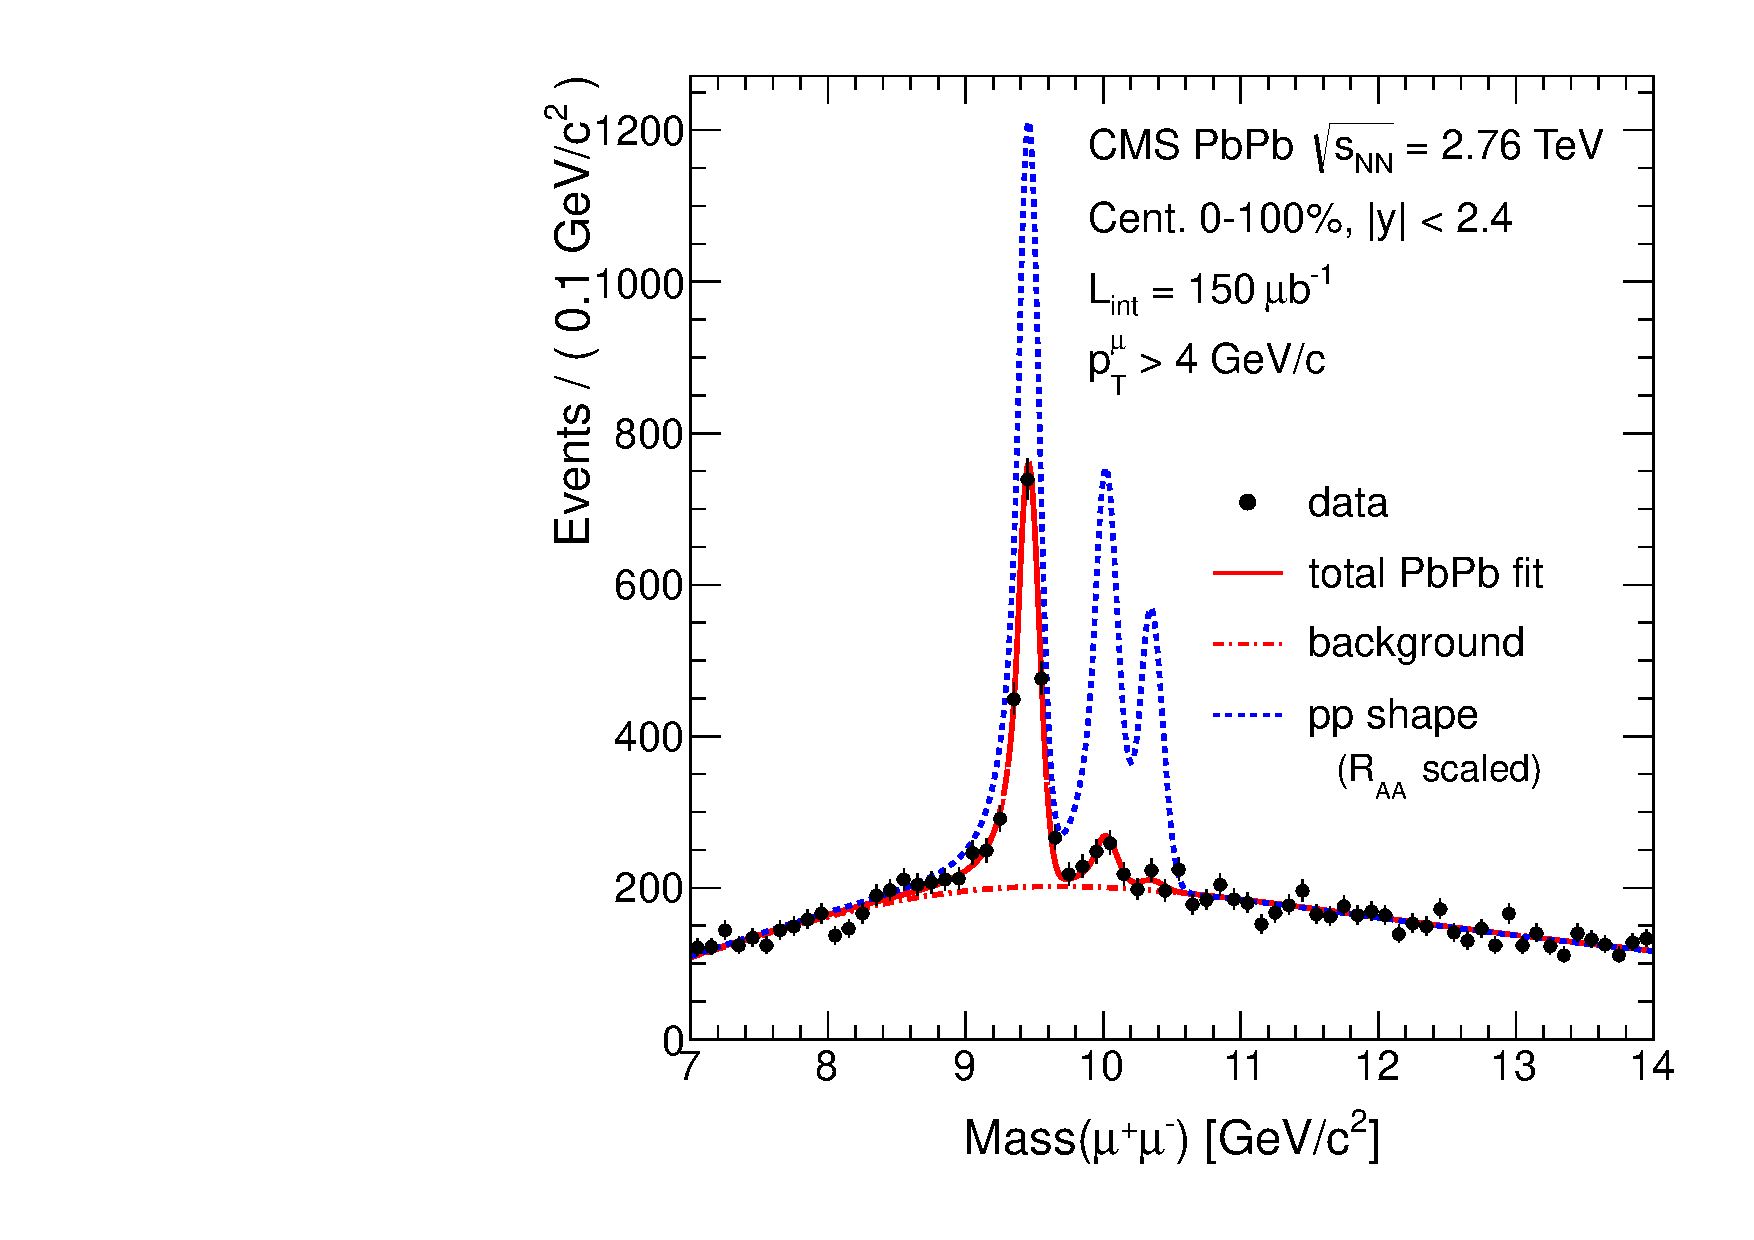
\includegraphics[height=0.4\textheight]{Chapters/pQuarkonia/simultaneousfit2011.pdf}
  \caption{The simultaneous fit of $pp$ and PbPb data recorded by CMS in the \PgU~mass
    range, exhibiting a clear suppression of the excited states. From~\cite{11-011}.}
  \label{fig:hinupsilons}
\end{center}
\end{figure}



Fortunately, the \PgU~mesons benefit from a larger mass, and one could
hope for many effects to either turn off or being still very small in
the presently analysed data. In the case of recombination for
example, it can be argued that not more than 2$\sim$5 $b\bar{b}$ pairs
can be formed in a central heavy ion collision~\cite{Denterria:2007xr}: as a result, the
recombination effect should be negligible, until a sufficient energy
density is reached.%  Moreover, the higher mass
% should also lead to a better comparison with perturbative effects, so
% the \PgU~calculations in cold nuclear matter should be more accurate,
% or just simpler, than what they are for \Jpsi.




% Turning to the dissociation temperature in the plasma, it is
% often argued that quarkonia are good probes of the plasma. If this
% proves to be 
% true, one would need to measure all the spectrum down to \pt\ = 0.

% Unfortunately, the fate of a static
% quarkonium in the QGP is unclear.
% Attempts are made to
% adress this point, and they tend to predict a \pt-dependent
% suppression, quickly growing to no suppression at intermediate or high momenta. In
% the case of \Jpsi, this would be complicated by the fact that nuclear
% absorption, in-medium parton energy loss and nuclear shadowing should be
% larger when the charmonium is at forward rapidity or small transverse
% momentum, but with the interplay of effects, it is unconclusive. In
% the case of \PgU~mesons however, given the higher quark mass, the
% binding of the potential \textit{and} the dissociation for various
% effects should be easier to model, putting the \PgU~to the front stage
% of QGP probes. We shall see in the following Chapters what is the
% result of such a measurement.



Recent results from the CMS collaboration~\cite{torsten,HIN-11-007,11-011} have reported a strong
suppression in the \PgU~decay to two muons, with a relatively small
$pp$ reference, giving quite large normalisation uncertainties. A measurement of
\PgU\ dimuon mass distributions in $pp$ and PbPb is presented in Figure~\ref{fig:hinupsilons}, where
the invariant mass plots for $pp$ and PbPb data are displayed in a
simultaneous fit exhibiting the observed PbPb suppression. On
Figure~\ref{fig:hinupsilonsraa} the centrality dependence of the suppression is
presented for \PgUa~and \PgUb, hinting at an ordered pattern, while
the \PgUc~remains unobserved in PbPb.
\\
Since then, a larger $pp$ reference dataset has been recorded by CMS,
allowing for a more precise measurement in centrality, and opening for
the possibility of a kinematic measurement of the suppression. This is
the topic covered in the present document. The following Chapters
will present the experimental setup and techniques put in place to
measure the \PgU~suppression in PbPb with a new level of precision.
\begin{figure}[t]
\begin{center}
  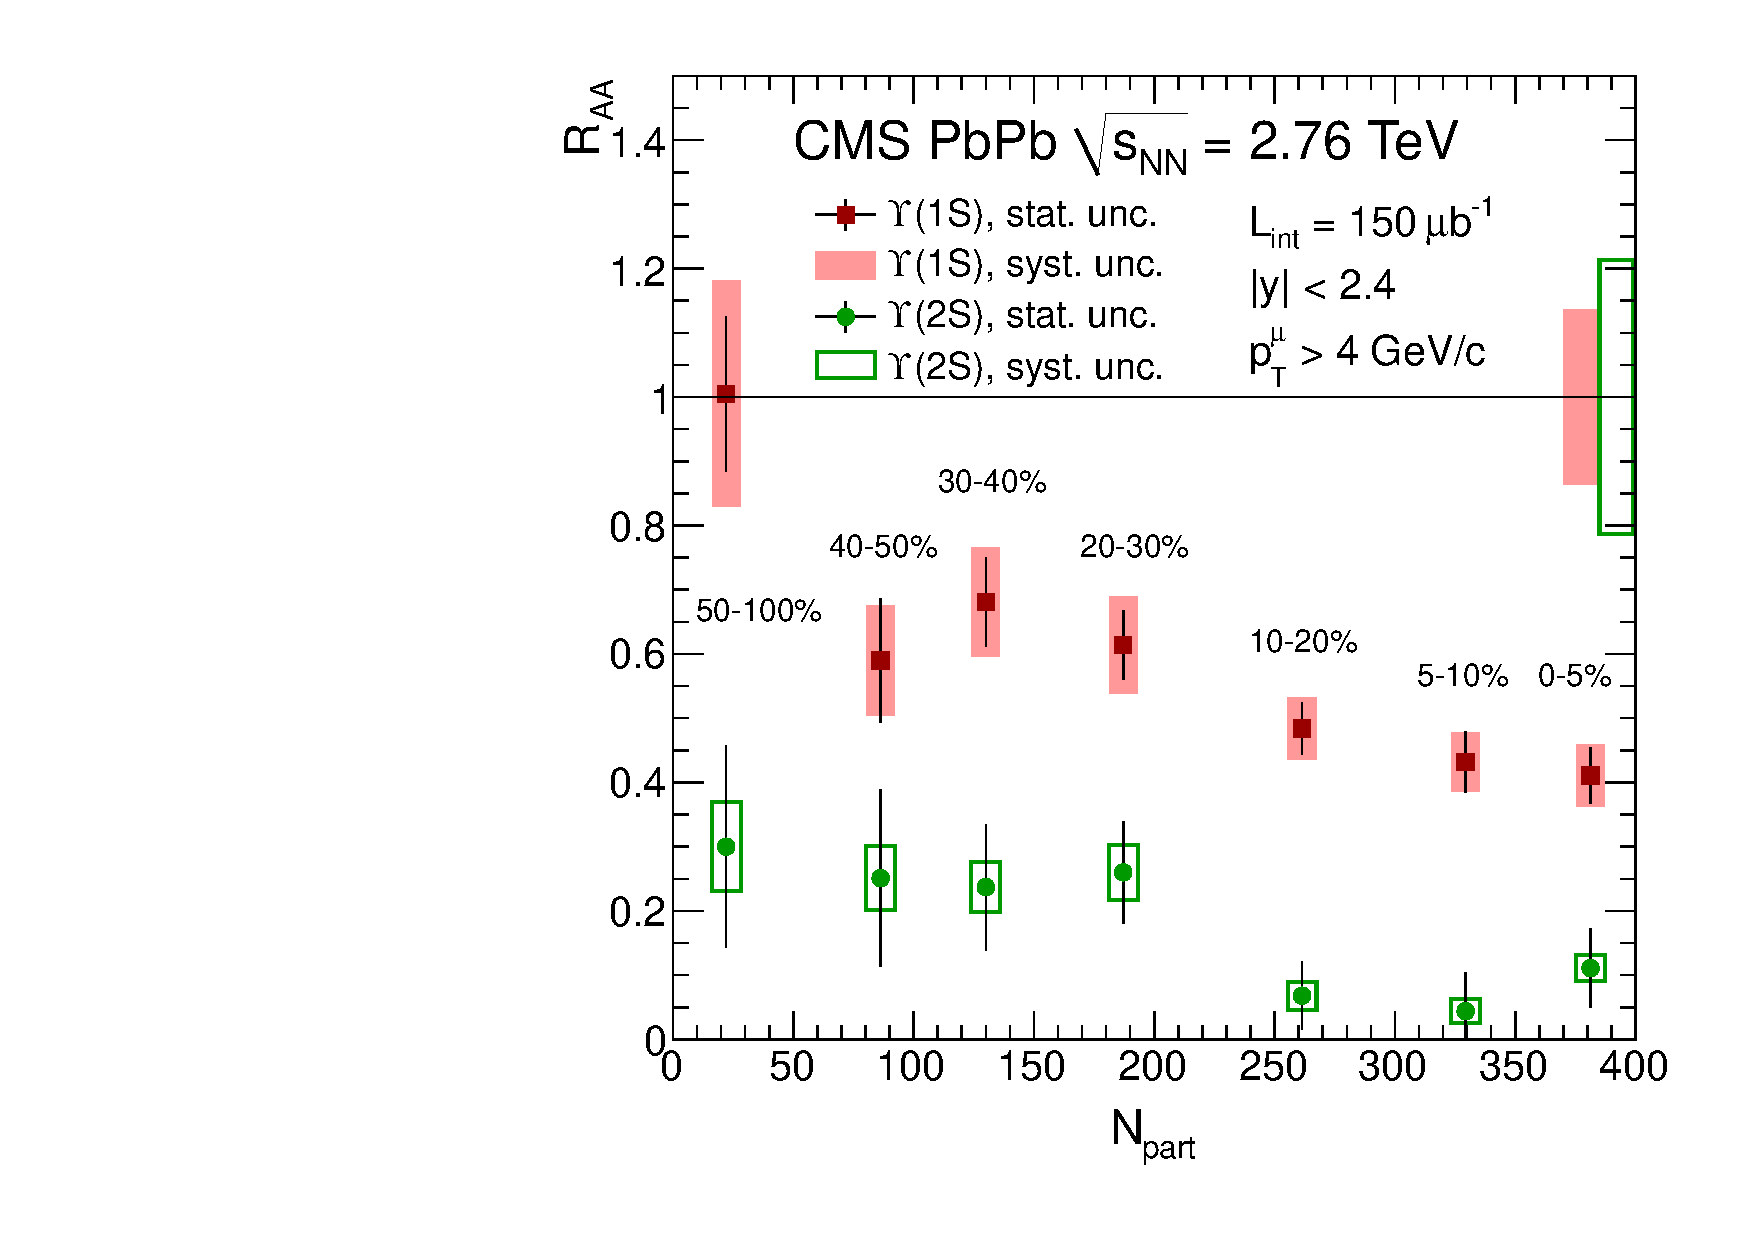
\includegraphics[height=0.4\textheight]{Chapters/pQuarkonia/RaaPt4.pdf}
  \caption{CMS measurement of the centrality dependence of \PgUa\ and
    \PgUb\ suppression in PbPb
    collisions at \snn\ = 2.76 TeV. From~\cite{11-011}.}
  \label{fig:hinupsilonsraa}
\end{center}
\end{figure}



\vspace{0.5em}
\begin{center}
  \fbox{
    \parbox{0.9\textwidth}
    {\textsf {In this Chapter, I have presented the basics of
        quarkonium measurements at hadron colliders. I have laid out
        the main results of the search for deconfinement in the
        quarkonium sector, and presented the state of the art of
        quarkonium measurements in $pp$ and PbPb data at the time of
        the beginning of this thesis. In 2013, a large $pp$ reference dataset has been recorded by CMS,
allowing for a more precise measurement in centrality, and opening for
the possibility of a kinematic measurement of the suppression.}}} 
\end{center}

